\documentclass{article}
\usepackage{cite}
\usepackage{amsmath,amssymb,amsfonts}
\usepackage{graphicx}
\usepackage{calc}
\usepackage{textcomp}
\usepackage[justification=centering]{caption}
\usepackage[justification=centering]{subcaption}
\usepackage[font=footnotesize]{caption}
\usepackage{float}
\usepackage{pifont}
\usepackage{algorithm}
\usepackage{algpseudocode}
\usepackage{multicol}
\usepackage{mathtools}
\usepackage{tabularray}
\usepackage{forloop}
\usepackage{pgffor}
\usepackage{stackengine}
\usepackage{xcolor}
\definecolor{Links}{HTML}{7A0022}
\usepackage{hyperref}
\hypersetup{
    colorlinks=true,
    citecolor=Links,
    linkcolor=Links,
    filecolor=Links,      
    urlcolor=Links,
    pdftitle={Triangular Automata: The 256 Elementary Cellular Automata of the 2D Plane},
    pdfpagemode=FullScreen,
}

\newcommand*{\Scale}[2][4]{\scalebox{#1}{\ensuremath{#2}}}%
  
\def\BibTeX{{\rm B\kern-.05em{\sc i\kern-.025em b}\kern-.08em
    T\kern-.1667em\lower.7ex\hbox{E}\kern-.125emX}}
    
\providecommand{\keywords}[1]
{
  \small	
  \textbf{\textit{Keywords ---}} #1
}
    
\begin{document}

\title{\Huge Triangular Automata \\
\Large The 256 Elementary Cellular Automata of the 2D Plane}

\author{Paul Cousin \\
        \small Université Paris Cité, France
}

\date{}

\maketitle

\begin{abstract}
Triangular Automata (TA) stands for cellular automata in the triangular grid. This work focuses on the simplest type of TA called Elementary Triangular Automata (ETA). They are argued to be the two-dimensional counterpart of Wolfram's Elementary Cellular Automata. Conceptual and computational tools for their study are presented along with an initial analysis. The paper is accompanied by a website where the results can be explored interactively. The source code is available in the form of a Mathematica package. \smallskip
\end{abstract} 

\keywords{cellular automata, triangular grid, dynamical systems, complexity.}

\vspace{20pt}

\section{Preamble} \label{preamble}
This paper comes with a website where you can interactively explore the 256 cellular automata presented here (including through different kinds of animations), as well as an easy-to-use Mathematica package.

\begin{enumerate}
    \item[•]\hspace{-1.5mm} Website: \href{https://paulcousin.github.io/triangular-automata}{paulcousin.github.io/triangular-automata}
    \item[•]\hspace{-1.5mm} Package demonstration: \href{https://paulcousin.github.io/triangular-automata-mathematica}{paulcousin.github.io/triangular-automata-mathematica}
\end{enumerate}

\section{Introduction} \label{introduction}
Cellular automata in the triangular grid, or \textbf{Triangular Automata} (TA) for short, have already been studied in a few papers \cite{
gerlingClassificationTriangularHoneycomb1990,
baysCellularAutomataTriangular1994,
imaiComputationuniversalTwodimensional8state2000,
naumovGeneralizedCoordinatesCellular2003,
linApplicationUnstructuredCellular2009,
baysCellularAutomataTriangular2009,
baysGameLifeNonsquare2010,
zawidzkiApplicationSemitotalistic2D2011,
brecklingCellularAutomataEcological2011,
saadatCellularAutomataTriangular2016,
ortigozaACFUEGOSUnstructuredTriangular2016,
uguzStructureReversibility2D2017,
saadatCellularAutomataApproach2018,
wainerIntroductionCellularAutomata2019,
pavlovaUsingCellularAutomata2020,
saadatGeneratingPatternsTriangular2021,
saadatCopyMachinesSelfreproduction2023}. This work will focus on a natural subset of TA called \textbf{Elementary Triangular Automata} (ETA). 

\begin{figure}[H]
    \centering
    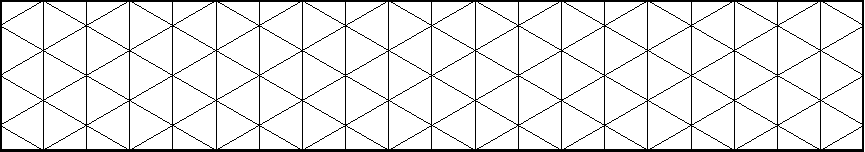
\includegraphics[width=.75\textwidth]{graphics/introduction/grid.pdf}
    \caption{The triangular grid}
    \label{fig:triangular-grid}
\end{figure}

\noindent ETA cells hold only \textbf{binary states}, each cell will thus either be:
\begin{enumerate}
    \item[•] ``alive" and colored purple \raisebox{-0.2\height}{
\includegraphics[height=3mm]{graphics/introduction/purple.pdf}}, with a state $s=1$ 
    \item[•] ``dead" and colored white \raisebox{-0.2\height}{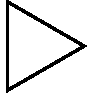
\includegraphics[height=3mm]{graphics/introduction/white.pdf}}  with a state $s=0$
\end{enumerate}
\  \\
ETA \textbf{rules} determine the future state of a cell based on its current state and the states of its neighbors, regardless of their orientation. This results in only 8 possible local configurations.

\begin{figure}[H]
     \centering
     \hfill
     \begin{subfigure}[b]{0.1\textwidth}
         \centering
         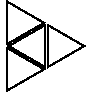
\includegraphics[width=\textwidth]{graphics/introduction/configurations/c0.pdf}
         \caption*{0}
     \end{subfigure}
     \hfill
     \begin{subfigure}[b]{0.1\textwidth}
         \centering
         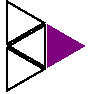
\includegraphics[width=\textwidth]{graphics/introduction/configurations/c1.pdf}
         \caption*{1}
     \end{subfigure}
     \hfill
     \begin{subfigure}[b]{0.1\textwidth}
         \centering
         
\includegraphics[width=\textwidth]{graphics/introduction/configurations/c2.pdf}
         \caption*{2}
     \end{subfigure}
     \hfill
     \begin{subfigure}[b]{0.1\textwidth}
         \centering
         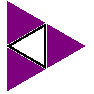
\includegraphics[width=\textwidth]{graphics/introduction/configurations/c3.pdf}
         \caption*{3}
     \end{subfigure}
     \hfill
     \begin{subfigure}[b]{0.1\textwidth}
         \centering
         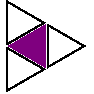
\includegraphics[width=\textwidth]{graphics/introduction/configurations/c4.pdf}
         \caption*{4}
     \end{subfigure}
     \hfill
     \begin{subfigure}[b]{0.1\textwidth}
         \centering
         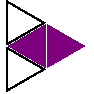
\includegraphics[width=\textwidth]{graphics/introduction/configurations/c5.pdf}
         \caption*{5}
     \end{subfigure}
     \hfill
     \begin{subfigure}[b]{0.1\textwidth}
         \centering
         
\includegraphics[width=\textwidth]{graphics/introduction/configurations/c6.pdf}
         \caption*{6}
     \end{subfigure}
     \hfill
     \begin{subfigure}[b]{0.1\textwidth}
         \centering
         
\includegraphics[width=\textwidth]{graphics/introduction/configurations/c7.pdf}
         \caption*{7}
     \end{subfigure}
     \hfill
     \caption{All possible local configurations}
        \label{fig:configurations}
\end{figure}

This paper uses a graph-theoretical framework developed in a previous work on Graph-Rewriting Automata\cite{cousin2022organic}. The triangular grid will here be considered as a graph (\textit{Figure \ref{fig:structure-of-the-triangular-grid}}). This graph must be expanded at each time step to simulate an infinite grid. The \textbf{region of influence} of a single cell grows in hexagonal layers (\textit{Figure \ref{fig:layers}}). This is therefore the most efficient way to expand the graph as well. How to do this in practice will be detailed in \textit{Section \ref{growing-the-grid}}.

\begin{figure}[H]
     \centering
     \begin{subfigure}[b]{0.40\textwidth}
         \centering
         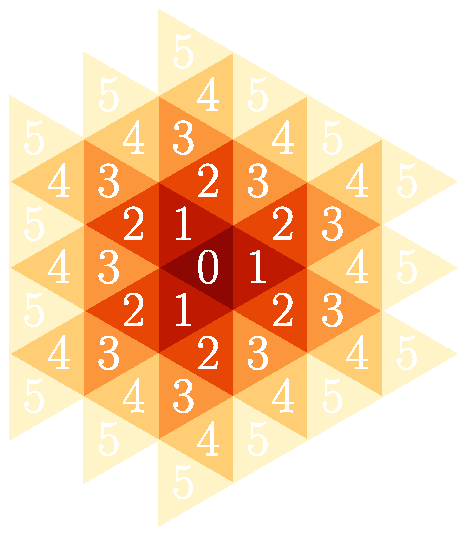
\includegraphics[width=\textwidth]{graphics/introduction/layers.pdf}
         \caption{Grid and layers}
         \label{fig:layers}
     \end{subfigure}
     \hspace{0.05\textwidth}
     \begin{subfigure}[b]{0.35\textwidth}
         \centering
         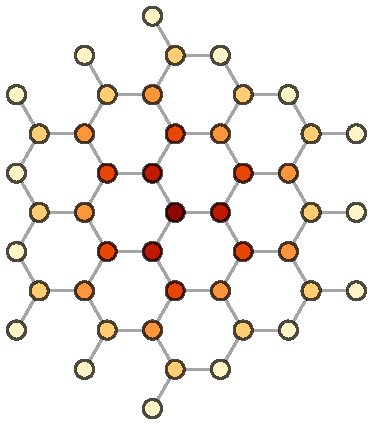
\includegraphics[width=\textwidth]{graphics/introduction/graph.pdf}
         \caption{Corresponding graph}
         \label{fig:graph}
     \end{subfigure}
        \caption{Structure of the triangular grid}
        \label{fig:structure-of-the-triangular-grid}
\end{figure}

 It is useful to see the triangular grid as a graph because computing the evolution of ETA is made quite easy by properties of its \textbf{adjacency matrix} $\mathcal{A}$ and \textbf{state}\linebreak\textbf{vector} $\mathcal{S}$. Every \textbf{vertex} $v$ of this graph will hold a \textbf{state} $s(v)$. The \textbf{neighborhood} $N(v)$ of a vertex is defined as the set of its adjacent vertices.
\begin{equation}
\begin{array}{ccc}
    \mathcal{A}_{ij}=
    \begin{cases}
        1 & \text{ if } v_i\in N(v_j) \\
        0 & \text{ otherwise}
    \end{cases}
&\hspace{1cm}&
    \mathcal{S}_i=s(v_i)\in\{0,1\}
\end{array}
\end{equation}

The \textbf{configuration} $c(v)$ of a vertex is a number which, when they are indexed as in \linebreak \textit{Figure \ref{fig:configurations}}, can be expressed as follows:
\begin{equation}
c(v)=4\times s(v)+\sum_{i\in N(v)} s(i)
\end{equation}

The space of possible ETA rules is finite. For each one of the 8 configurations, a rule must specify whether the vertex will be dead or alive at $t+1$. Consequently, there are only $2^8=256$ possible rules. For this reason, ETA can be seen as the two-dimensional counterpart of Wolfram’s 256 Elementary Cellular Automata\cite{wolfram2002new, weisstein2002elementary}. Furthermore, the triangle is the regular polygon tiling 2D space with the smallest number of neighbors per cell. ETA are thus the most basic 2D cellular automata and have a fundamental aspect in this regard. \\

\noindent Each \textbf{rule} $R$ is a map from \textbf{configuration space} to \textbf{state space}.
\begin{equation}
\begin{aligned}
& R: \{0,1,2,3,4,5,6,7\}\rightarrow\{0,1\}\\  
& R\big(c_t(v)\big)=s_{t+1}\big(v\big)
\end{aligned}
\end{equation}

Each rule can be labeled by a unique \textbf{rule number} $n$ (see \textit{Equation \ref{eq:rule-number}}). We will use the labeling system which was independently proposed in \cite{zawidzkiApplicationSemitotalistic2D2011} and \cite{cousin2022organic}, since it must be somewhat natural and because it has useful properties. This system, inspired by the Wolfram code \cite{wolfram2002new}, is such that a rule number in its binary form displays the behavior of the rule. Starting from the right, its digits indicate the future state for each configuration as they have been ordered previously. \textit{Figure \ref{fig:rule-plot-181}} shows the example of rule 181.

\begin{equation} \label{eq:rule-number}
    n=\sum_{i=0}^7 2^i R(i)
\end{equation}

\begin{figure}[H]
    \centering
    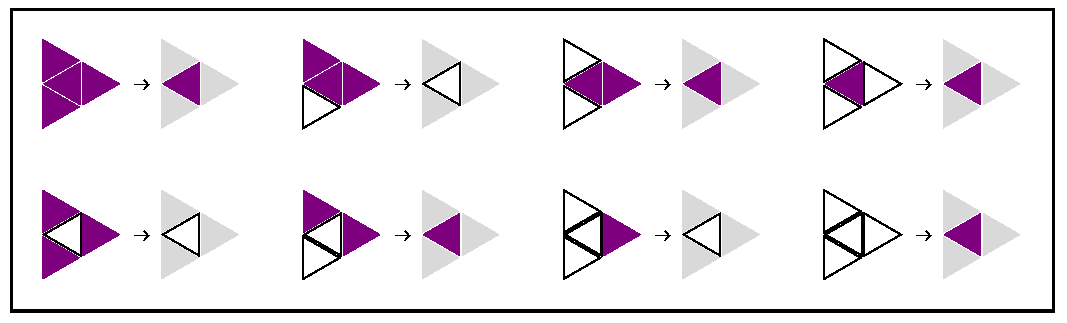
\includegraphics[width=.8\textwidth]{graphics/introduction/rule-plot-181.pdf}
    \caption{Rule $181=1011,0101_2$}
    \label{fig:rule-plot-181}
\end{figure}

\section{Behavior} \label{behavior}
Before going into the details of how to compute these automata, we can take a look at how they behave. In this section, a preliminary study of ETA will be presented to motivate a future, more in-depth analysis. It is of particular interest to see what happens to a single living cell under different ETA rules so, unless otherwise noted, the following figures come from this starting point.

\pagebreak
\subsection{Beauty} \label{beauty}
One of the most striking aspects of these automata is their aesthetic quality, which cannot be better illustrated than by a few selected examples.

\begin{figure}[H]
    \centering
    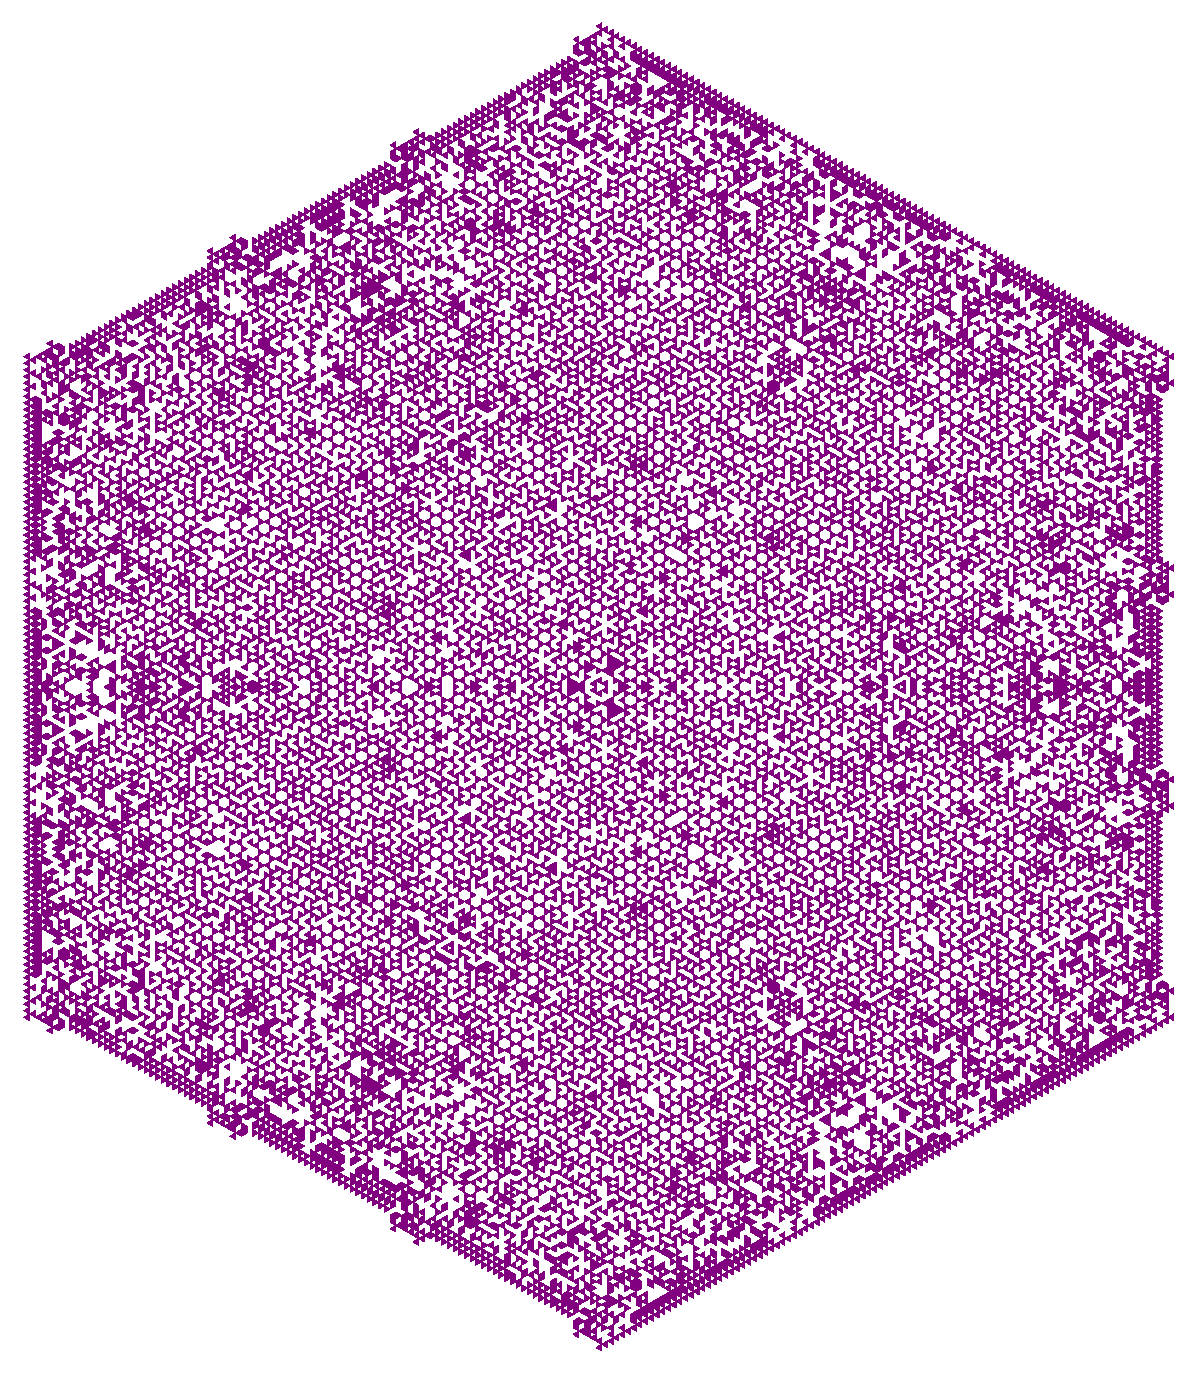
\includegraphics[width=.59\textwidth]{graphics/behavior/beauty/rule-89-time-200-OneAlive.pdf}
    \caption{Rule 89 at $t=200$}
    \label{fig:rule-89-time-200-OneAlive}
\end{figure}
\begin{figure}[H]
    \centering
    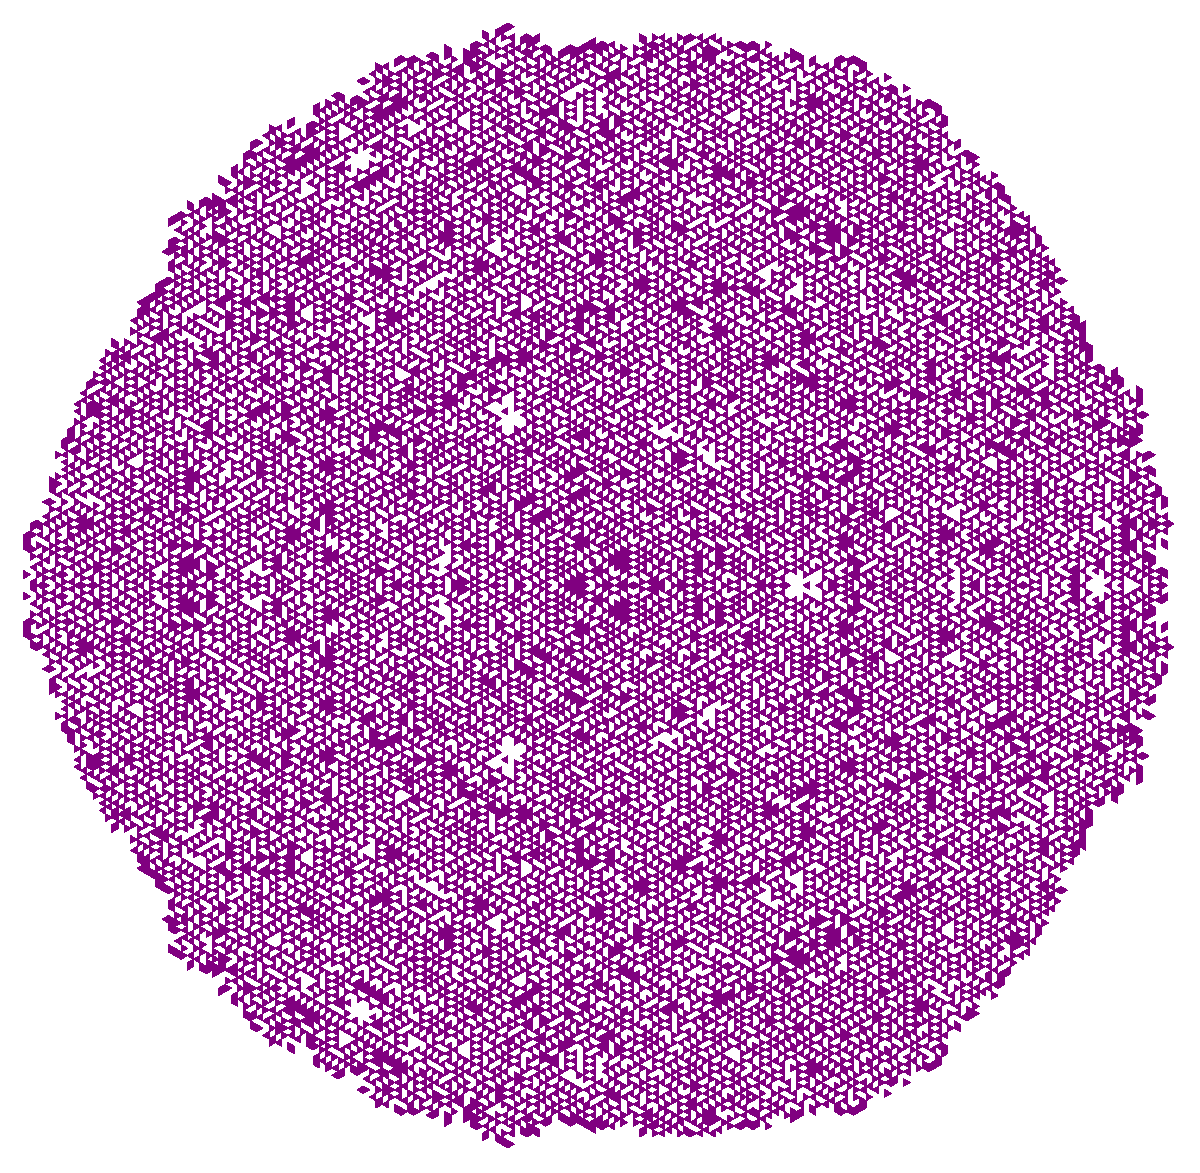
\includegraphics[width=.59\textwidth]{graphics/behavior/beauty/rule-57-time-320-OneAlive.pdf}
    \caption{Rule 57 at $t=320$}
    \label{fig:rule-57-time-320-OneAlive}
\end{figure}

\begin{figure}[H]
    \centering
    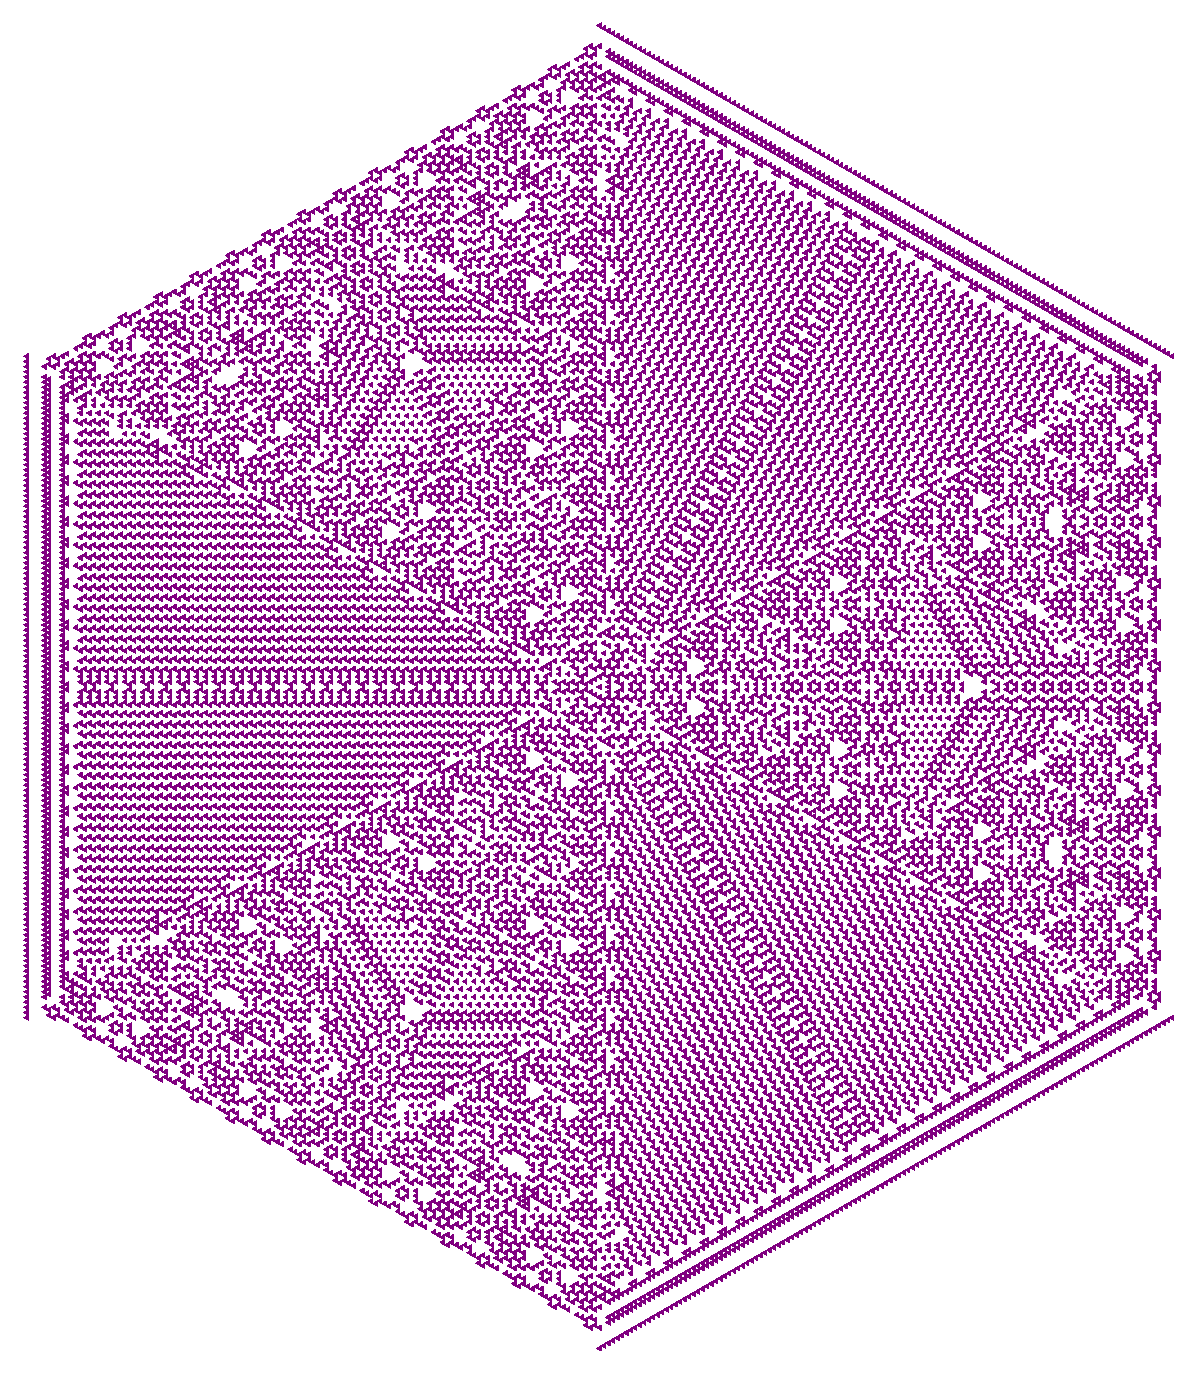
\includegraphics[width=.618\textwidth]{graphics/behavior/beauty/rule-73-time-256-OneAlive.pdf}
    \caption{Rule 73 at $t=256$}
    \label{fig:rule-73-time-256-OneAlive}
\end{figure}
\begin{figure}[H]
    \centering
    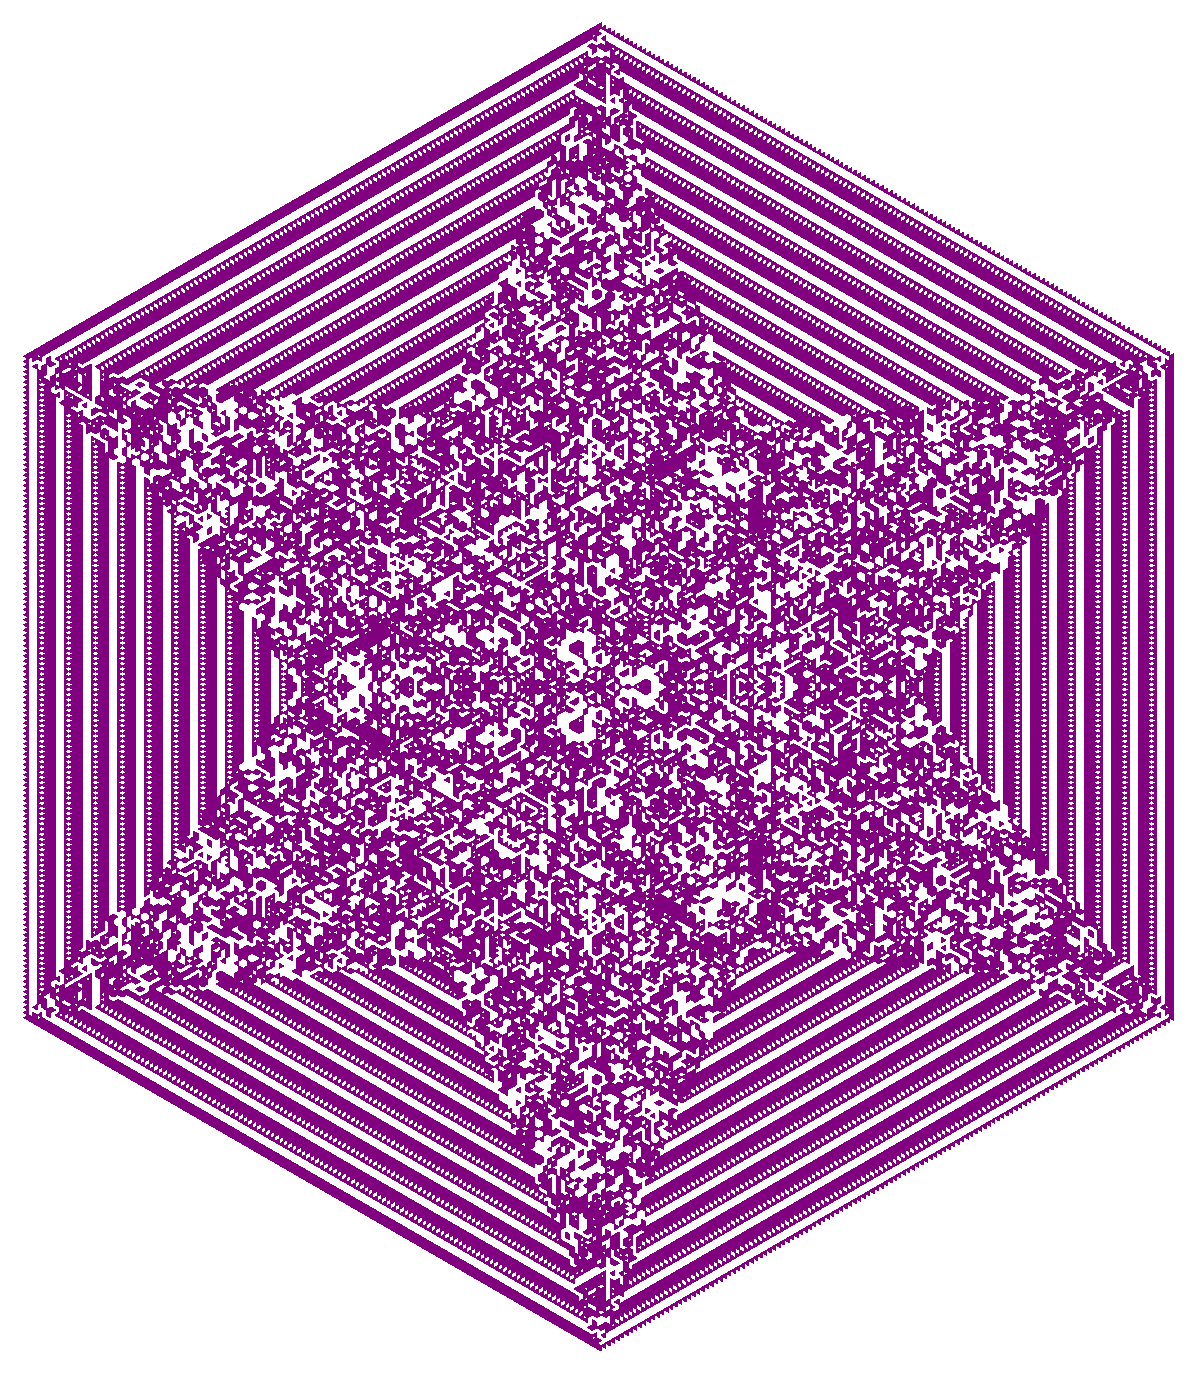
\includegraphics[width=.618\textwidth]{graphics/behavior/beauty/rule-62-time-256-OneAlive.pdf}
    \caption{Rule 62 at $t=256$}
    \label{fig:rule-62-time-256-OneAlive}
\end{figure}

\subsection{Chaos} \label{chaos}
Given the existing literature on cellular automata, it is quite expected to see some of these rules behave chaotically. The example of rule 53 confirms it. Starting from two randomly generated 64 layers wide grids that are completely similar except for the central cell which is alive in (1) and dead in (2), the trajectories strongly diverge.

\bigskip

\begin{figure}[H]
     \centering
     \begin{subfigure}[b]{0.3\textwidth}
         \centering
         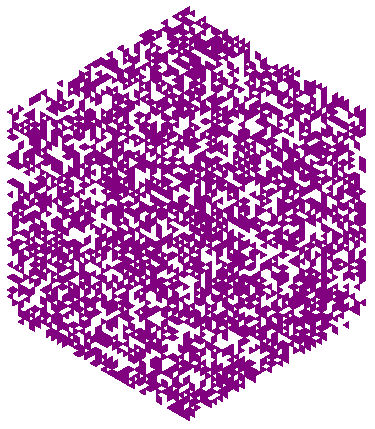
\includegraphics[width=\textwidth]{graphics/behavior/chaos/chaos-1-1.pdf}
         \caption*{(1) at $t=0$}
     \end{subfigure}
     \hspace{0.17\textwidth}
     \begin{subfigure}[b]{0.3\textwidth}
         \centering
         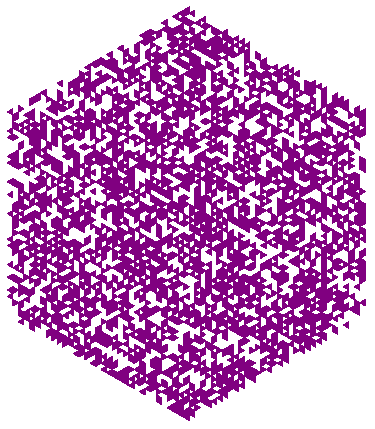
\includegraphics[width=\textwidth]{graphics/behavior/chaos/chaos-2-1.pdf}
         \caption*{(2) at $t=0$}
     \end{subfigure}
    \break\vspace{5mm}
     \begin{subfigure}[b]{0.48\textwidth}
         \centering
         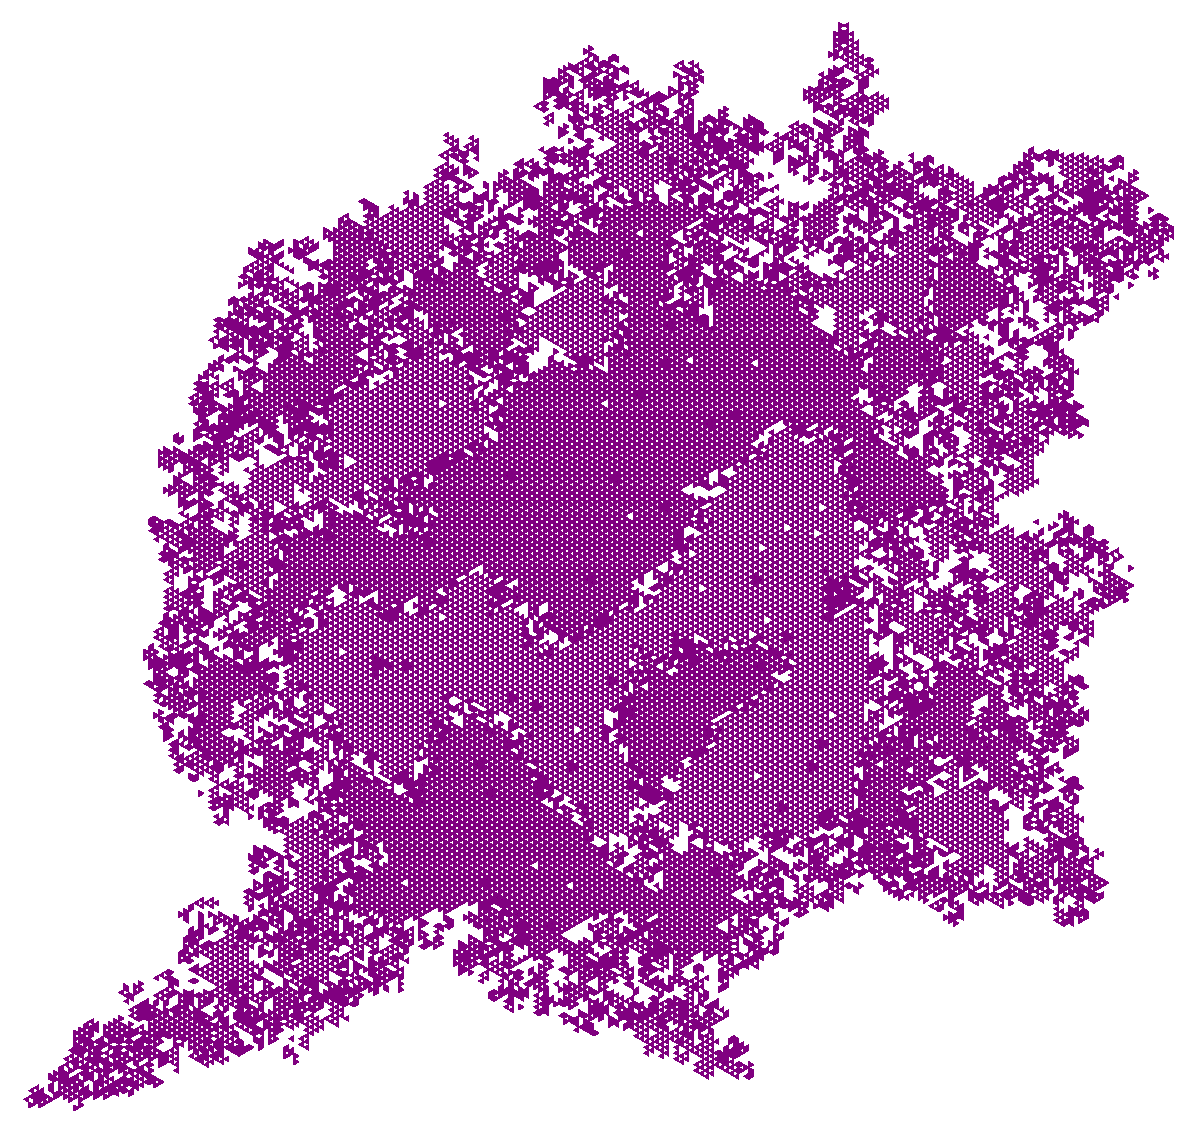
\includegraphics[width=\textwidth]{graphics/behavior/chaos/chaos-1-2.pdf}
         \caption*{(1) at $t=512$}
     \end{subfigure}
     \begin{subfigure}[b]{0.48\textwidth}
         \centering
         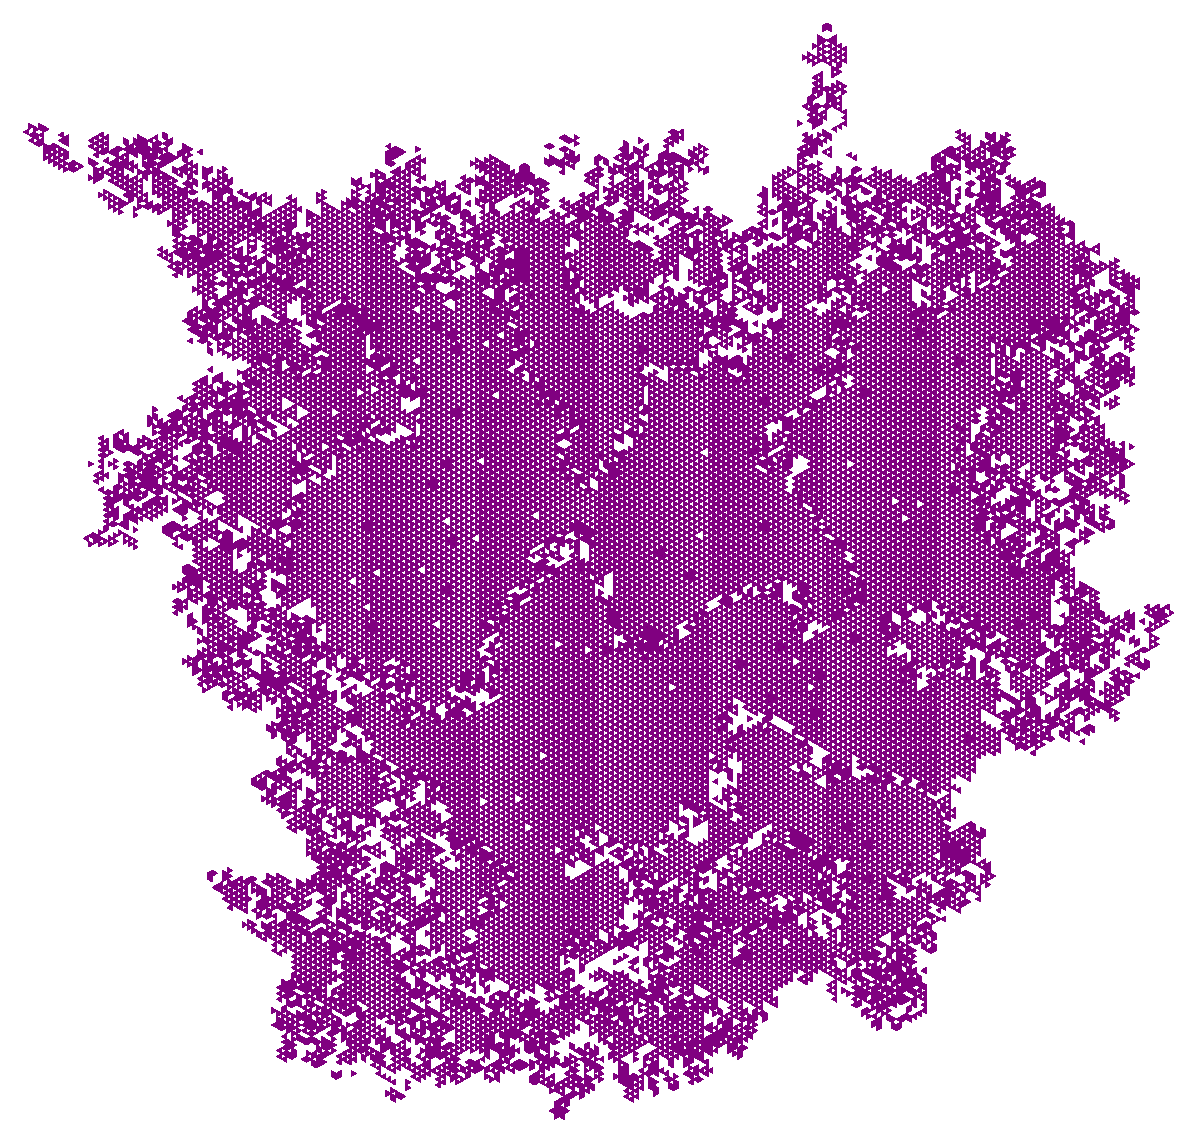
\includegraphics[width=\textwidth]{graphics/behavior/chaos/chaos-2-2.pdf}
         \caption*{(2) at $t=512$}
     \end{subfigure}
     \caption{Chaotic behavior of rule 53}
        \label{fig:chaos}
\end{figure}

\bigskip

\begin{figure}[H]
    \centering
        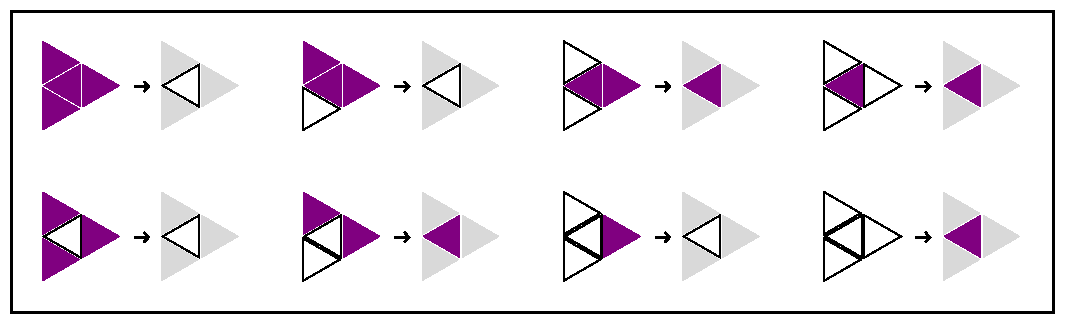
\includegraphics[width=.7\textwidth]{graphics/behavior/chaos/rule-53.pdf}
    \caption{Rule 53}
    \label{fig:rule-plot-53}
\end{figure}

\pagebreak
\subsection{Fractals} \label{fractals}
Some ETA rules produce remarkable scale-free structures. 

\begin{figure}[H]
    \centering
    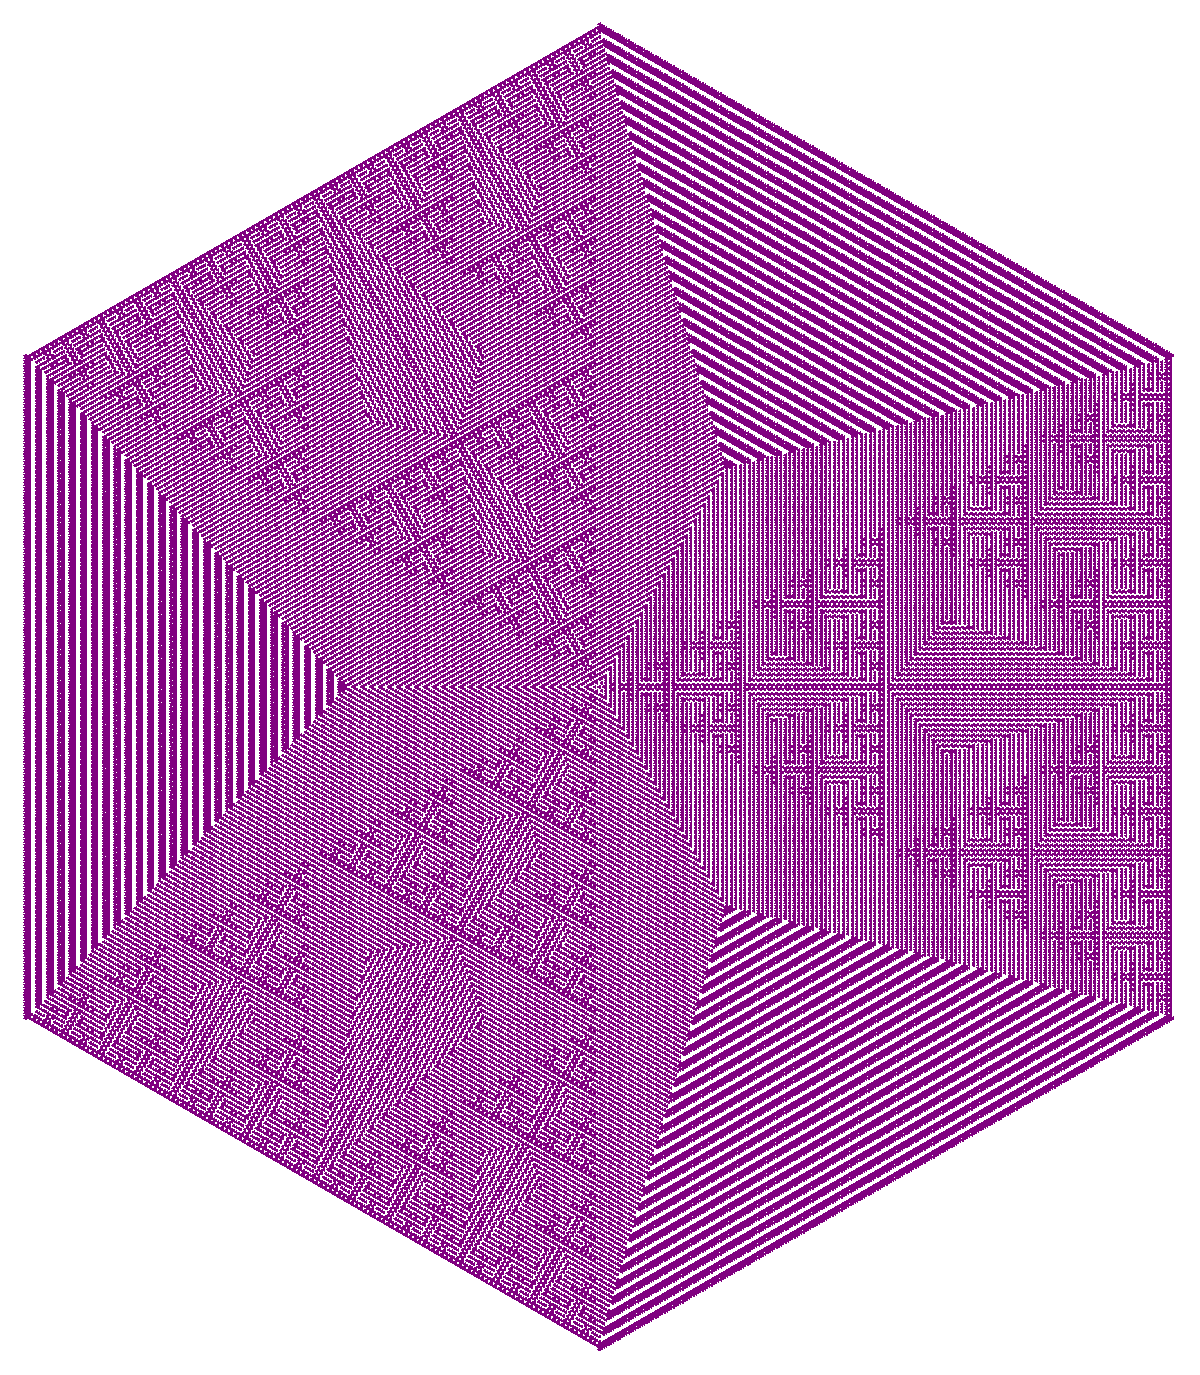
\includegraphics[width=.58\textwidth]{graphics/behavior/fractals/rule-65-time-512-OneAlive.pdf}
    \caption{Rule 65 at $t=512$}
    \label{fig:rule-65-time-512-OneAlive}
\end{figure}
\begin{figure}[H]
    \centering
    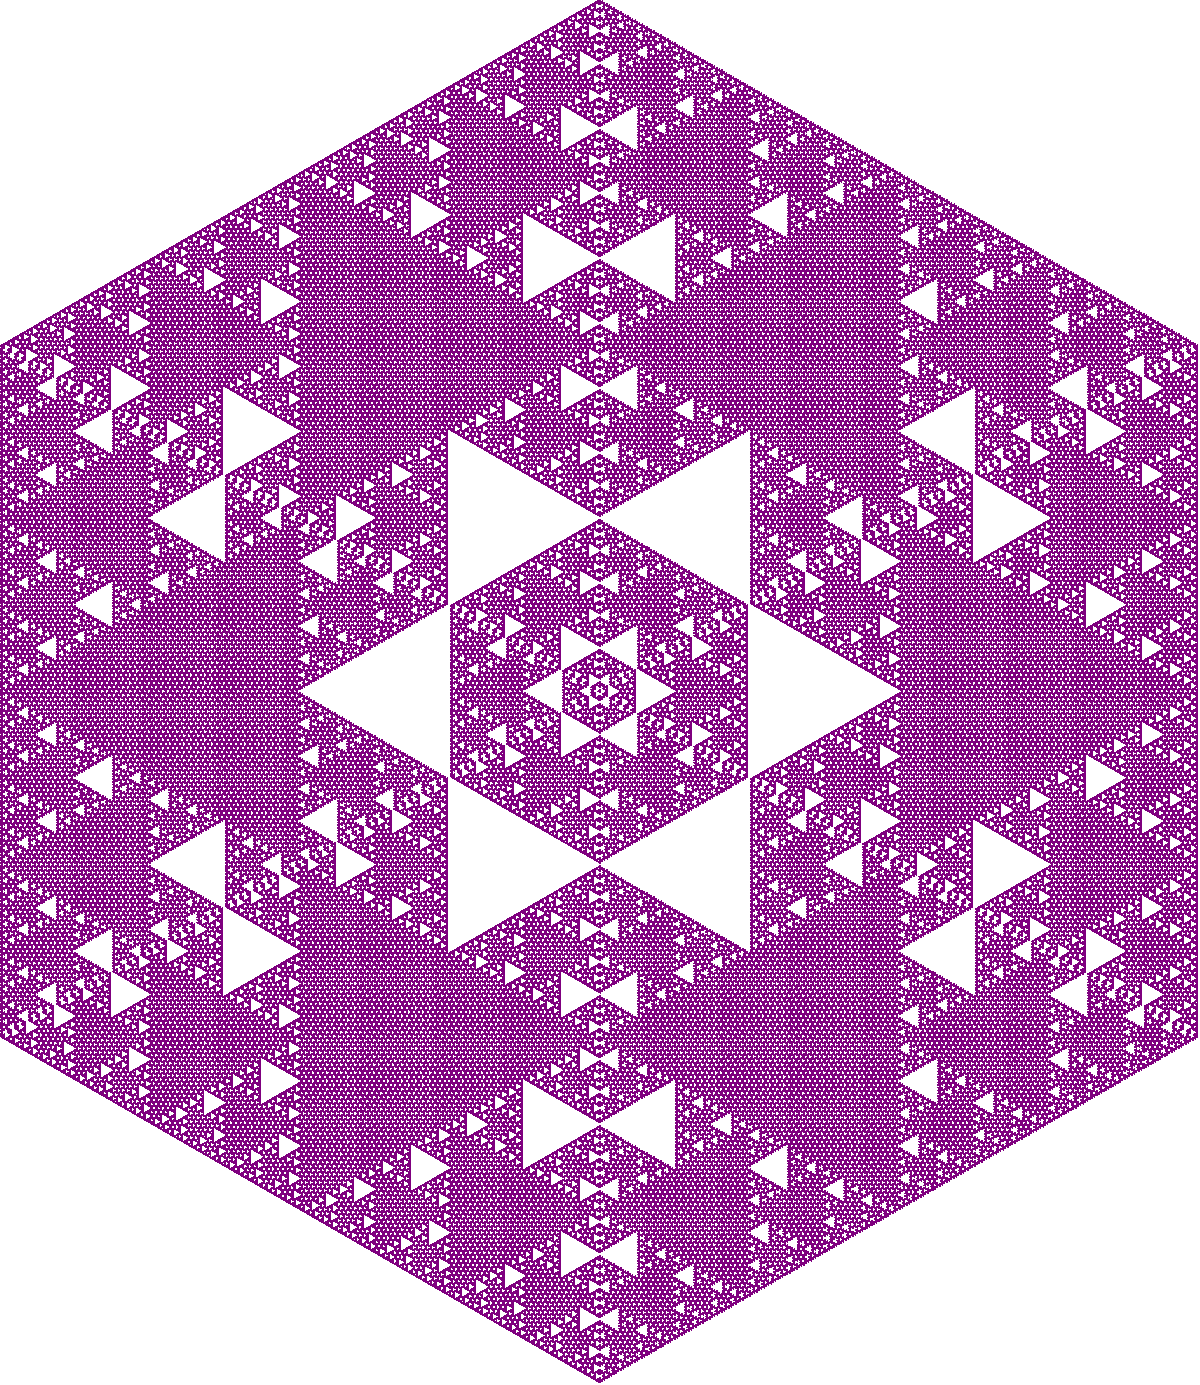
\includegraphics[width=.64\textwidth]{graphics/behavior/fractals/rule-106-time-510-OneAlive.pdf}
    \caption{Rule 106 at $t=510$}
    \label{fig:rule-106-time-510-OneAlive}
\end{figure}

\pagebreak
\ \\
\vspace{5mm}

\begin{figure}[H]
    \centering
    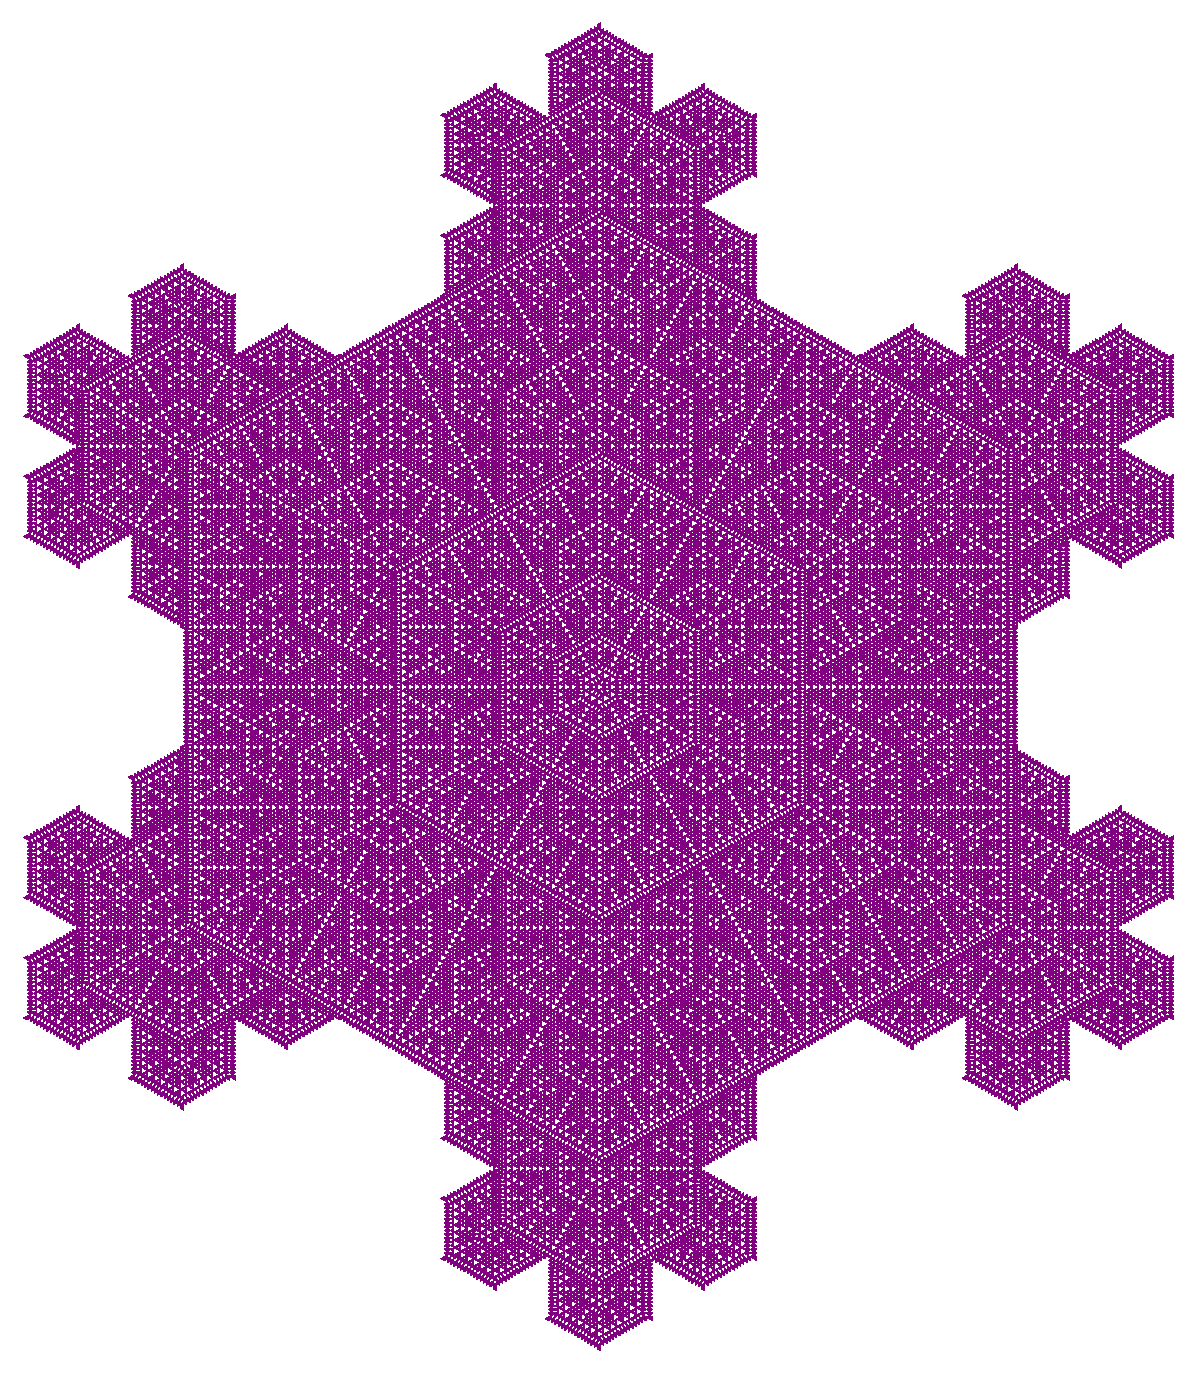
\includegraphics[width=\textwidth]{graphics/behavior/fractals/rule-50-time-352-OneAlive.pdf}
    \caption{Rule 50 at $t=352$}
    \label{fig:rule-50-time-352-OneAlive}
\end{figure}

\pagebreak
\subsection{Space-Time} \label{space-time}
Similar to the way Elementary Cellular Automata \cite{wolfram2002new, weisstein2002elementary} are most often represented, the evolution of an ETA can be displayed in one single plot. Here, an instant is two-dimensional, so adding the dimension of time creates a 3D structure. In these \textbf{space-time plots}, time flows downward. The successive grids are stacked beneath each other, starting from the initial conditions at the top. To avoid the infinite planes created by an alive environment, we can display only the cells that have the opposite state to it at each time step. A lot of information is therefore lost. We do not see most of the internal structure and we cannot know the state of the environment. Nevertheless, this representation helps visualize some properties of ETA that are difficult to notice otherwise. For instance, certain rules create 3D space-time fractals.

\vspace{1cm}

\begin{figure}[H]
    \centering
    \includegraphics[width=\textwidth]{graphics/behavior/space-time/rule-10-perspective.jpg}
    \caption{Space-time plot of rule 10 up to $t=512$}
    \label{fig:rule-10-perspective}
\end{figure}

% \pagebreak
% \ \\
% \vspace{1cm}

% \begin{figure}[H]
%     \centering
%     \includegraphics[width=\textwidth]{graphics/behavior/space-time/rule-10-orthographic.jpg}
%     \caption{Space-time plot of rule 10 up to $t=512$ (orthographic)}
%     \label{fig:rule-10-orthographic}
% \end{figure}



\pagebreak
\subsection{Center Column} \label{center-column}
\noindent There are a few rules where the state of the first living cell evolves in an interesting way. This sequence of states forms the center column of the space-time plots.
\vspace{40pt}

\begin{figure}[H]
    \centering
    \begin{subfigure}[b]{0.49\textwidth}
        \centering
        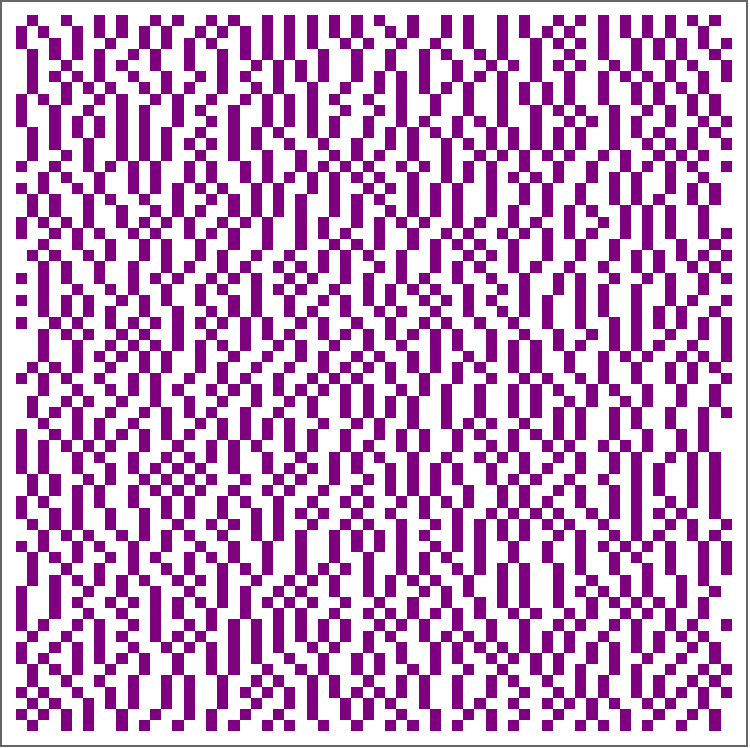
\includegraphics[width=.8\textwidth]{graphics/behavior/center-columns/rule-37-center_column_plot-4096.pdf}
        \caption{Rule 37 (OEIS \href{https://oeis.org/A371844}{A371844})}
        \label{fig:rule-37-center_column_plot-4096}
    \end{subfigure}
    \vspace{16pt}
    \begin{subfigure}[b]{0.49\textwidth}
        \centering
        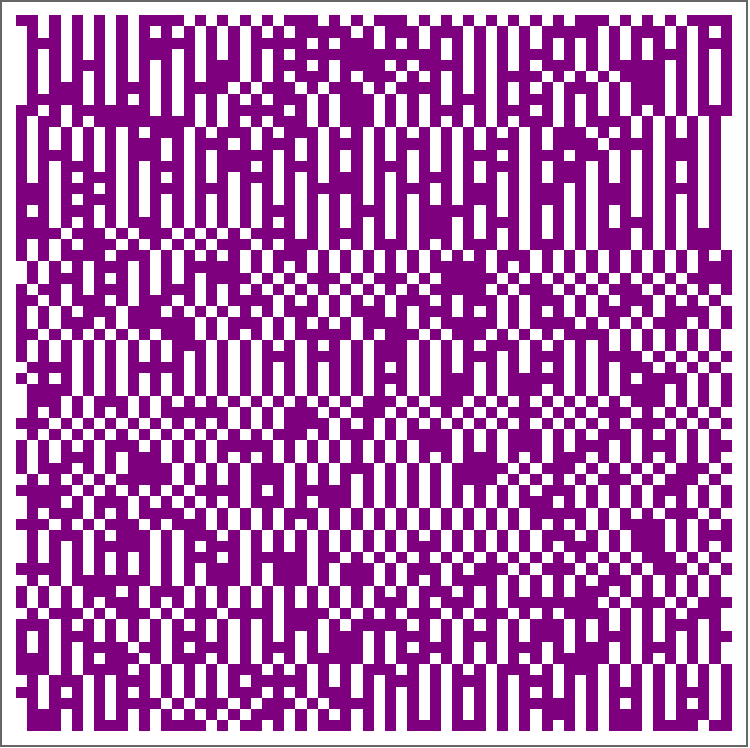
\includegraphics[width=.8\textwidth]{graphics/behavior/center-columns/rule-61-center_column_plot-4096.pdf}
        \caption{Rule 61 (OEIS \href{https://oeis.org/A372553}{A372553})}
        \label{fig:rule-61-center_column_plot-4096}
    \end{subfigure}
    \begin{subfigure}[b]{0.49\textwidth}
        \centering
        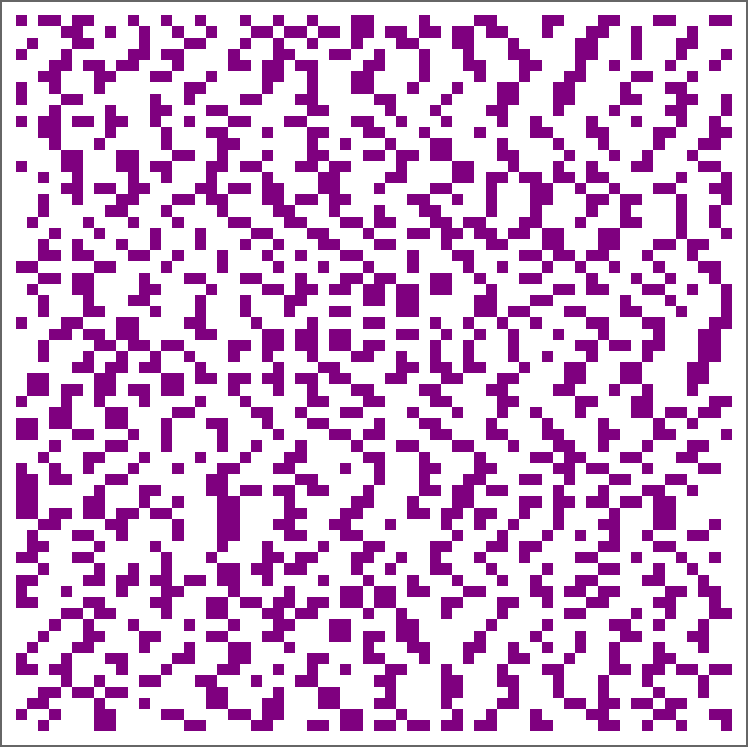
\includegraphics[width=.8\textwidth]{graphics/behavior/center-columns/rule-62-center_column_plot-4096.pdf}
        \caption{Rule 62 (OEIS \href{https://oeis.org/A371931}{A371931})}
        \label{fig:rule-62-center_column_plot-4096}
    \end{subfigure}
    \vspace{4pt}
    \begin{subfigure}[b]{0.49\textwidth}
        \centering
        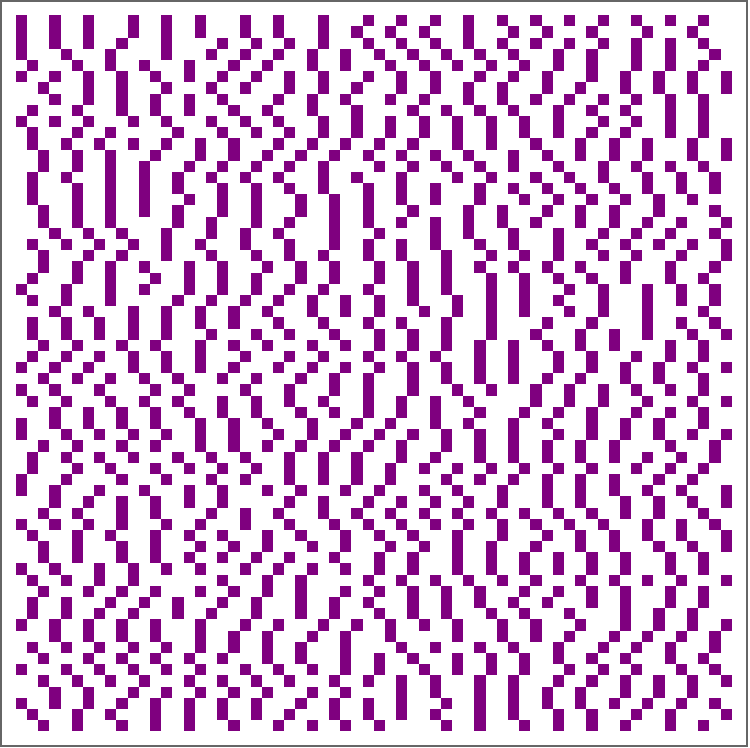
\includegraphics[width=.8\textwidth]{graphics/behavior/center-columns/rule-94-center_column_plot-4096.pdf}
        \caption{Rule 94 (OEIS \href{https://oeis.org/A372552}{A372552})}
        \label{fig:rule-94-center_column_plot-4096}
    \end{subfigure}
       \caption{Center columns $1\leq t \leq 4096$ (read left-to-right, top-to-bottom)}
       \label{fig:center-columns}
\end{figure}


\pagebreak
\subsection{Self-Reproduction} \label{self-reproduction}

As mentioned in \cite{saadatCopyMachinesSelfreproduction2023}, one of the original motivations for the development of cellular automata was to create a mathematical model of self-reproduction. Interestingly, 4 of the 256 ETA rules naturally reproduce any finite pattern given as initial conditions: rules 85, 90, 165 and 170. A proof of self-reproduction based on path counting already exists for rule 170 \cite{saadatCopyMachinesSelfreproduction2023}. Similarly spirited proofs could probably be proposed for the others.

\vspace{.6cm}

\begin{table}[H]
    \centering
    \begin{tblr}{|Q[c,m]|Q[c,h] Q[c,h] Q[c,h] Q[c,h]|}
        \hline
            t & rule 85 & rule 90 & rule 165 & rule 170 \\
        \hline
            0 &
            \raisebox{-.05\height}{
\includegraphics[width=0.19\textwidth]{graphics/behavior/self-reproduction/rule-85-time-0.pdf}} &
            \raisebox{-.05\height}{
\includegraphics[width=0.19\textwidth]{graphics/behavior/self-reproduction/rule-90-time-0.pdf}} &
            \raisebox{-.05\height}{
\includegraphics[width=0.19\textwidth]{graphics/behavior/self-reproduction/rule-165-time-0.pdf}} &
            \raisebox{-.05\height}{
\includegraphics[width=0.19\textwidth]{graphics/behavior/self-reproduction/rule-170-time-0.pdf}} \\
            16 &
            \raisebox{-.05\height}{
\includegraphics[width=0.19\textwidth]{graphics/behavior/self-reproduction/rule-85-time-16.pdf}} &
            \raisebox{-.05\height}{
\includegraphics[width=0.19\textwidth]{graphics/behavior/self-reproduction/rule-90-time-16.pdf}} &
            \raisebox{-.05\height}{
\includegraphics[width=0.19\textwidth]{graphics/behavior/self-reproduction/rule-165-time-16.pdf}} &
            \raisebox{-.05\height}{
\includegraphics[width=0.19\textwidth]{graphics/behavior/self-reproduction/rule-170-time-16.pdf}} \\
            32 &
            \raisebox{-.05\height}{
\includegraphics[width=0.19\textwidth]{graphics/behavior/self-reproduction/rule-85-time-32.pdf}} &
            \raisebox{-.05\height}{
\includegraphics[width=0.19\textwidth]{graphics/behavior/self-reproduction/rule-90-time-32.pdf}} &
            \raisebox{-.05\height}{
\includegraphics[width=0.19\textwidth]{graphics/behavior/self-reproduction/rule-165-time-32.pdf}} &
            \raisebox{-.05\height}{
\includegraphics[width=0.19\textwidth]{graphics/behavior/self-reproduction/rule-170-time-32.pdf}} \\
            48 &
            \raisebox{-.05\height}{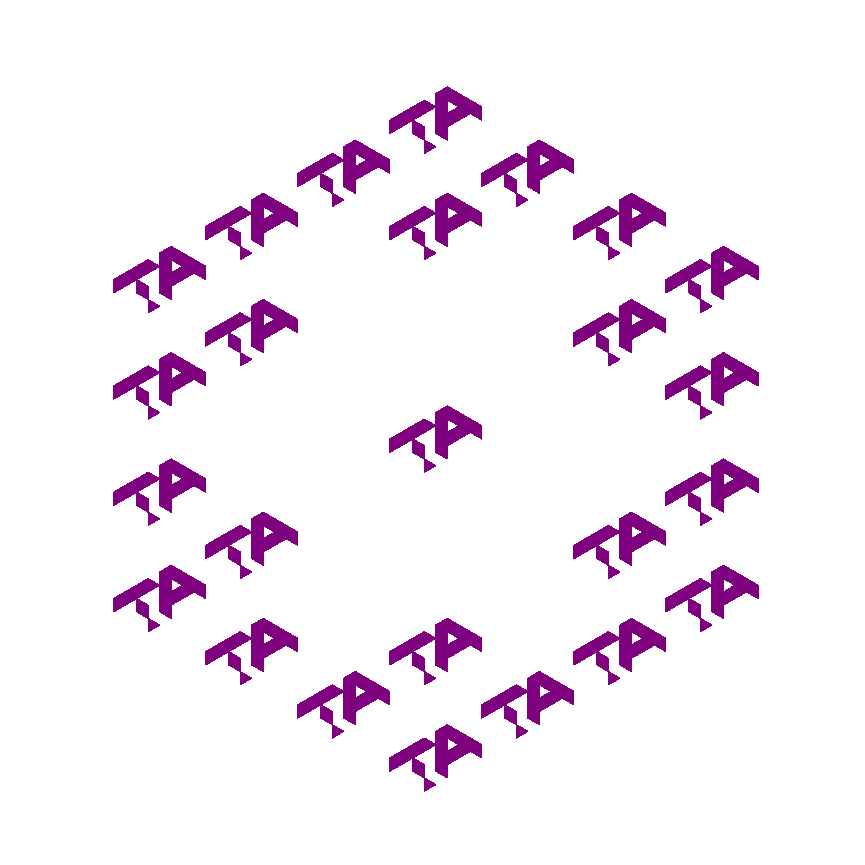
\includegraphics[width=0.19\textwidth]{graphics/behavior/self-reproduction/rule-85-time-48.pdf}} &
            \raisebox{-.05\height}{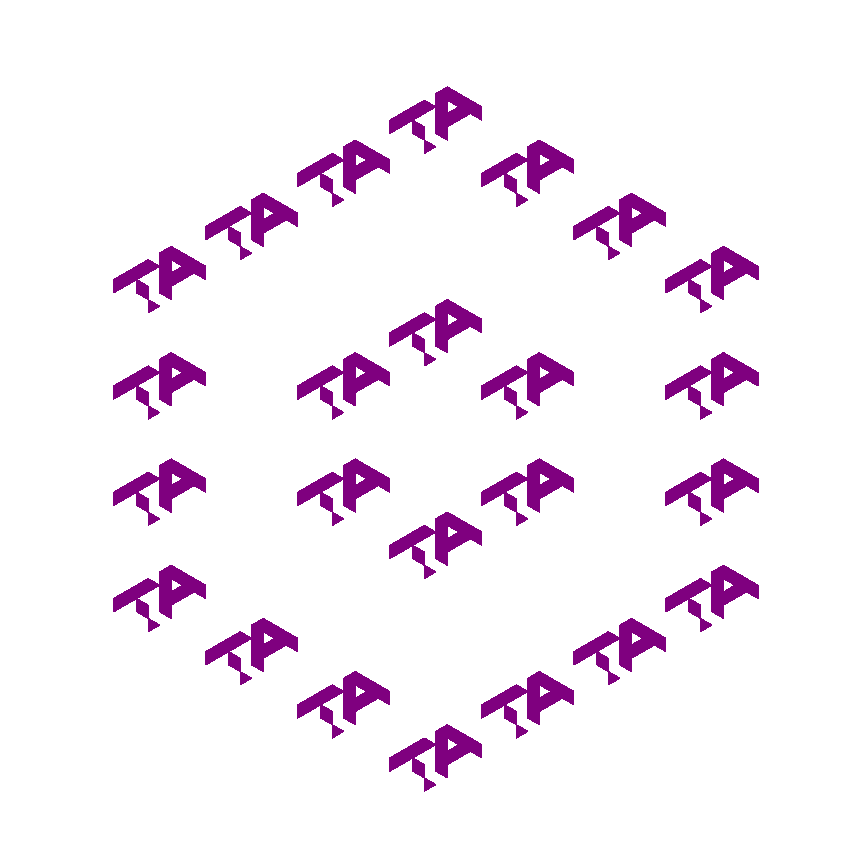
\includegraphics[width=0.19\textwidth]{graphics/behavior/self-reproduction/rule-90-time-48.pdf}} &
            \raisebox{-.05\height}{
\includegraphics[width=0.19\textwidth]{graphics/behavior/self-reproduction/rule-165-time-48.pdf}} &
            \raisebox{-.05\height}{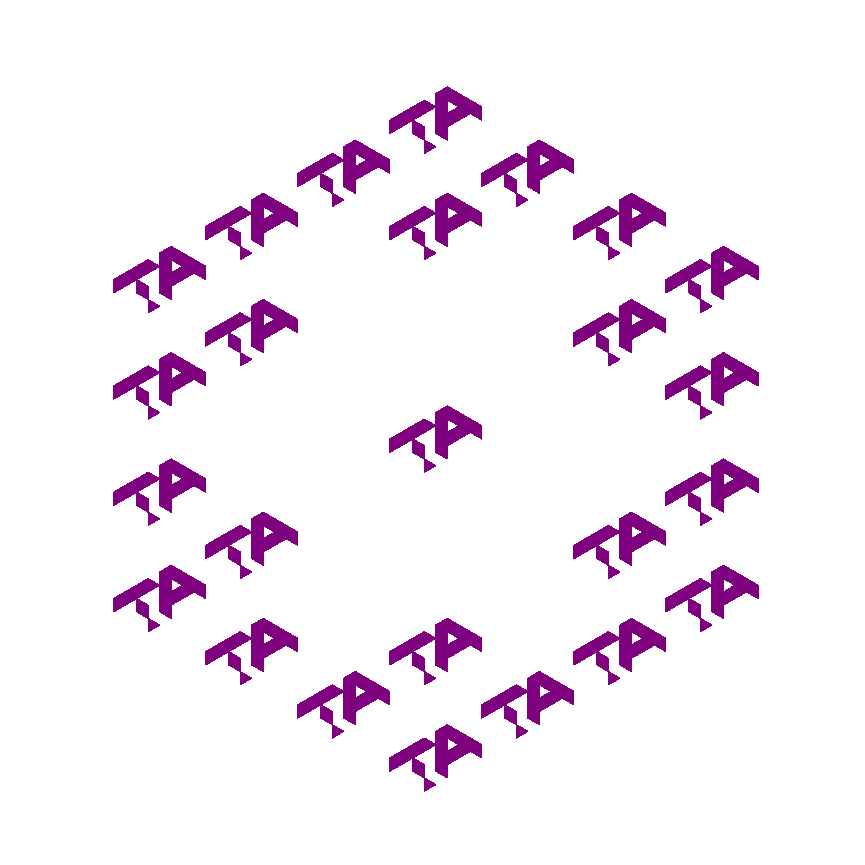
\includegraphics[width=0.19\textwidth]{graphics/behavior/self-reproduction/rule-170-time-48.pdf}} \\
            112 &
            \raisebox{-.05\height}{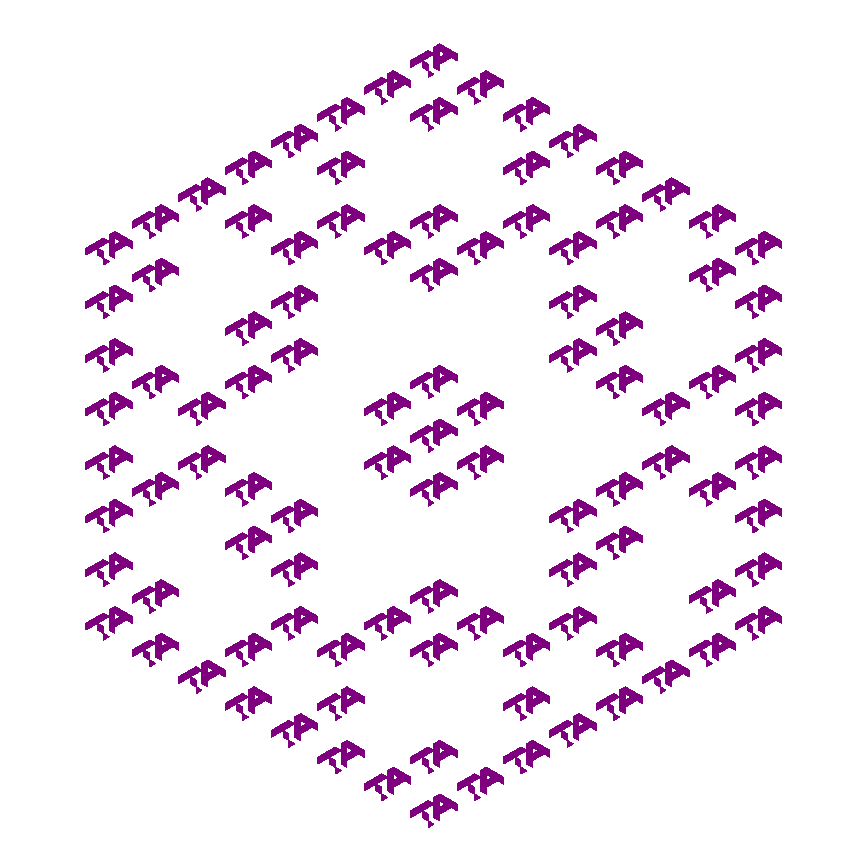
\includegraphics[width=0.19\textwidth]{graphics/behavior/self-reproduction/rule-85-time-112.pdf}} &
            \raisebox{-.05\height}{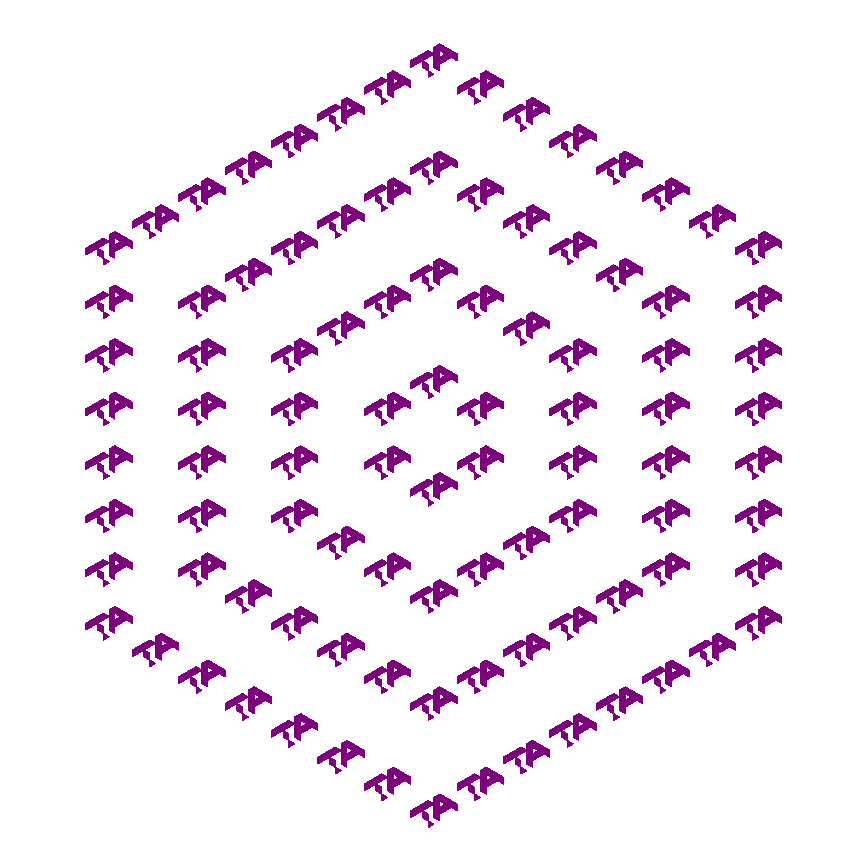
\includegraphics[width=0.19\textwidth]{graphics/behavior/self-reproduction/rule-90-time-112.pdf}} &
            \raisebox{-.05\height}{\includegraphics[width=0.19\textwidth]{graphics/behavior/self-reproduction/rule-165-time-112.pdf}} &
            \raisebox{-.05\height}{\includegraphics[width=0.19\textwidth]{graphics/behavior/self-reproduction/rule-170-time-112.pdf}} \vspace{0pt} \\ 
        \hline
    \end{tblr}
    \caption{Pattern self-reproduction from a recognizable starting point}
    \label{tab:my_label}
\end{table}


\pagebreak
\subsection{Rule 210} \label{rule-210}
Rule 210 is easy to describe: ``change the state of cells that have one neighbor alive". It is special for several reasons: it creates larger structures as time goes on and a new type of structure appears from around $t=1024$.


\begin{figure}[H]
    \centering
    \begin{tblr}{c c c c c}
            % \raisebox{-.05\height}{\includegraphics[width=0.165\textwidth]{graphics/behavior/rule-210/rule-210-time-256.jpg}} &
            % \raisebox{-.05\height}{\includegraphics[width=0.165\textwidth]{graphics/behavior/rule-210/rule-210-time-512.jpg}} &
            % \raisebox{-.05\height}{\includegraphics[width=0.165\textwidth]{graphics/behavior/rule-210/rule-210-time-1024.jpg}} &
            % \raisebox{-.05\height}{\includegraphics[width=0.165\textwidth]{graphics/behavior/rule-210/rule-210-time-2048.jpg}} &
            % \raisebox{-.05\height}{\includegraphics[width=0.165\textwidth]{graphics/behavior/rule-210/rule-210-time-4096.jpg}} \\
            % 256 & 512 & 1024 & 2048 & 4096 \\
            
            \raisebox{-.05\height}{\includegraphics[width=0.165\textwidth]{graphics/behavior/rule-210/rule-210-time-257.jpg}} &
            \raisebox{-.05\height}{\includegraphics[width=0.165\textwidth]{graphics/behavior/rule-210/rule-210-time-513.jpg}} &
            \raisebox{-.05\height}{\includegraphics[width=0.165\textwidth]{graphics/behavior/rule-210/rule-210-time-1025.jpg}} &
            \raisebox{-.05\height}{\includegraphics[width=0.165\textwidth]{graphics/behavior/rule-210/rule-210-time-2049.jpg}} &
            \raisebox{-.05\height}{\includegraphics[width=0.165\textwidth]{graphics/behavior/rule-210/rule-210-time-4097.jpg}} \\
            257 & 513 & 1025 & 2049 & 4097 \\
            
    \end{tblr}
    \caption{Rule 210 at $t=2^i +1$ (the structure is best seen on odd time steps from afar)}
    \label{tab:rule-210-evolution}
\end{figure}

\begin{figure}[H]
    \centering
    \includegraphics[width=.85\textwidth]{graphics/behavior/rule-210/rule-210-time-4097-contrast.jpg}
    \caption{Rule 210 at $t=4097$ with enhanced constrat}
    \label{fig:rule-210-time-4097}
\end{figure}

\begin{figure}[H]
    \centering
    \includegraphics[width=\textwidth]{graphics/behavior/rule-210/rule-210-time-2048-close-up.jpg}
    \vspace{-16pt}
    \caption{Close-up of rule 210 at $t=2048$}
    \label{fig:rule-210-close-up-2048}
\end{figure}
\vspace{-10pt}
\begin{figure}[H]
    \centering
    \includegraphics[width=\textwidth]{graphics/behavior/rule-210/rule-210-time-4096-close-up.jpg}
    \vspace{-16pt}
    \caption{Close-up of rule 210 at $t=4096$}
    \label{fig:rule-210-close-up-4096}
\end{figure}

\noindent Rule 210 initially alternates between what seems like 2 population densities (i.e. number of living cells / size of the first cell's region of influence). When the new structure appears, around $t=1024$, the population stabilizes in a density cycle of period 4 between slowly evolving values.

\begin{figure}[H]
    \centering
    \begin{subfigure}[b]{0.51\textwidth}
        \centering
        \includegraphics[width=\textwidth]{graphics/behavior/rule-210/rule-210-population-plot.pdf}
        \caption{Population (OEIS \href{https://oeis.org/A372581}{A372581})}
    \end{subfigure}
    \begin{subfigure}[b]{0.48\textwidth}
        \centering
        \includegraphics[width=\textwidth]{graphics/behavior/rule-210/rule-210-density-plot.pdf}
        \caption{Population density}
    \end{subfigure}
       \caption{Evolution of two coarse-grained values under rule 210}
       \label{fig:rule-210-coarse-grained}
\end{figure}


\pagebreak
\subsection{Noise} \label{noise}
Some rules seem to generate a pretty good noise. For example, if we pick a simple starting point without symmetries, rule 37 will usually turn it into an expanding disk with a random-looking interior.

\vspace{1cm}

\begin{figure}[H]
    \centering
    \includegraphics[width=.07\textwidth]{graphics/behavior/noise/rule-37-time-0-asymmetric.pdf}
    \caption{Simple asymmetric starting point}
    \label{fig:rule-37-time-0-asymmetric}
\end{figure}

\begin{figure}[H]
    \centering
    \includegraphics[width=.9\textwidth]{graphics/behavior/noise/rule-37-time-512-asymmetric.pdf}
    \caption{Result at $t=512$ with rule 37}
    \label{fig:rule-37-time-512-asymmetric}
\end{figure}


\pagebreak
\subsection{Textures} \label{textures}
Organic textures can be obtained by applying other rules to this pseudorandom grid.

\begin{figure}[H]
    \centering
    \begin{subfigure}[b]{0.8\textwidth}
        \centering
        \includegraphics[width=\textwidth]{graphics/behavior/textures/rule-204-time-32-noise.pdf}
        \caption{Rule 204 at at $t=32$}
        \label{fig:rule-204-time-32-noise}
    \end{subfigure}
    \vspace{20pt}
    \begin{subfigure}[b]{0.49\textwidth}
        \centering
        \includegraphics[width=\textwidth]{graphics/behavior/textures/rule-100-time-64-noise.pdf}
        \caption{Rule 100 at at $t=64$}
        \label{fig:rule-100-time-64-noise}
    \end{subfigure}
    \begin{subfigure}[b]{0.49\textwidth}
        \centering
        \includegraphics[width=\textwidth]{graphics/behavior/textures/rule-108-time-512-noise.pdf}
        \caption{Rule 108 at at $t=512$}
        \label{fig:rule-108-time-512-noise}
    \end{subfigure}
        \vspace{-10pt}
       \caption{Starting from \textit{Figure \ref{fig:rule-37-time-512-asymmetric}}}
       \label{fig:textures}
\end{figure}


\pagebreak
\subsection{Boring Rules} \label{boring-rules}
\noindent There is an \textbf{identity} rule which leaves any grid unchanged: rule 240.
\begin{figure}[H]
    \centering
        \includegraphics[width=.5\textwidth]{graphics/behavior/boring-rules/rule-240.pdf}
    \caption{Rule 240}
    \label{fig:rule-plot-240}
\end{figure}

\noindent And a \textbf{negative} rule that swaps alive and dead states: rule 15.
\begin{figure}[H]
    \centering
        \includegraphics[width=.5\textwidth]{graphics/behavior/boring-rules/rule-15.pdf}
    \caption{Rule 15}
    \label{fig:rule-plot-1(}
\end{figure}

\subsection{Twins} \label{twins}
A simple procedure can be followed to find the evil twin of a rule that has the same effect but in the negative world. To find it, take the number in its binary form (with the leading zeros needed for the number to be 8 digits long), swap ones and zeros and read it backwards. Let us take rule 214 as an example. \\

\begin{tabular}{l c r}
     First, find the binary form of the rule number, 
     & & $214=11010110_2$ \\
     then swap ones and zeros
     & & $00101001_2$ \\
     and finally reverse it.
     & & $10010100_2=148$
\end{tabular}

\begin{figure}[H]
     \centering
     \begin{subfigure}[b]{0.48\textwidth}
         \centering
         \includegraphics[width=\textwidth]{graphics/behavior/twins/rule-214-OneAlive.pdf}
         \caption{rule 214 from one living cell at $t=128$}
         \label{fig:twin-1}
     \end{subfigure}
     \hspace{0.02\textwidth}
     \begin{subfigure}[b]{0.48\textwidth}
         \centering
         \includegraphics[width=\textwidth]{graphics/behavior/twins/rule-148-OneDead.pdf}
         \caption{rule 148 from one dead cell at $t=128$}
         \label{fig:twin-2}
     \end{subfigure}
        \caption{Twin rules}
        \label{fig:twins}
\end{figure}


\pagebreak
\section{Implementation} \label{implementation}
\subsection{Tools}
% \noindent Let us start by defining a few useful operators and matrices.

\begin{enumerate}
\item 
$\diamond$ here represents an operator that joins matrices corner to corner.

\begin{equation}
\begin{pmatrix}
{\color{purple}a} 
\end{pmatrix}
\diamond
\begin{pmatrix}
{\color{red}b} & {\color{red}c} \\
{\color{red}d} & {\color{red}e}
\end{pmatrix}
\diamond
\begin{pmatrix}
{\color{orange}f} & {\color{orange}g} & {\color{orange}h} 
\end{pmatrix}
=
\begin{pmatrix}
 {\color{purple}a} & {\color{lightgray}0} & {\color{lightgray}0} & {\color{lightgray}0} & {\color{lightgray}0} & {\color{lightgray}0} \\
{\color{lightgray}0} & {\color{red}b} & {\color{red}c} & {\color{lightgray}0} & {\color{lightgray}0} & {\color{lightgray}0}\\
{\color{lightgray}0} & {\color{red}d} & {\color{red}e} & {\color{lightgray}0} & {\color{lightgray}0} & {\color{lightgray}0}\\
{\color{lightgray}0} & {\color{lightgray}0} & {\color{lightgray}0} & {\color{orange}f} & {\color{orange}g} & {\color{orange}h} 
\end{pmatrix}
\end{equation}

\item 
$^\searrow\,$ shifts diagonally the elements of a matrix and places the last row and column first.

\begin{equation}
\begin{pmatrix}
a & b & c & {\color{orange}d} \\
e & f & g & {\color{orange}h} \\
{\color{red}i} & {\color{red}j} & {\color{red}k}  & {\color{purple}l} 
\end{pmatrix}
^{\hspace{-1.5mm}\searrow}
=
\begin{pmatrix}
{\color{purple}l}  & {\color{red}i} & {\color{red}j} & {\color{red}k} \\
{\color{orange}d} & a & b & c \\
{\color{orange}h} & e & f & g \\
\end{pmatrix}
\end{equation}

\item 
@ will be an operator applying a function to every element of a matrix. 
\begin{equation}
f\text{@}
\begin{pmatrix}
a & b \\
c & d
\end{pmatrix}
=
\begin{pmatrix}
f(a) & f(b) \\
f(c) & f(d)
\end{pmatrix}
\end{equation}

\item 
$\mathbb{I}_i$ is the $i\times i$ identity matrix. $\mathbb{S}_i$ will be a $i\times (i+1)$ ``stairs" matrix.
\begin{equation}
    \mathbb{I}_1=
    \begin{pmatrix}
    {\color{purple}1}
    \end{pmatrix}
\qquad\quad\;
    \mathbb{I}_2=
    \begin{pmatrix}
    {\color{purple}1} & 0 \\
    0 & {\color{purple}1}
    \end{pmatrix}
\qquad\quad\;
    \mathbb{I}_3=
    \begin{pmatrix}
    {\color{purple}1} & 0 & 0 \\
    0 & {\color{purple}1} & 0 \\
    0 & 0 & {\color{purple}1} 
    \end{pmatrix}
\qquad\quad\;
    \hdots
\quad
\end{equation}
\begin{equation}
    \mathbb{S}_1=
    \begin{pmatrix}
    {\color{purple}1} & {\color{purple}1}
    \end{pmatrix}
\qquad
    \mathbb{S}_2=
    \begin{pmatrix}
    {\color{purple}1} & {\color{purple}1} & 0 \\
    0 & {\color{purple}1} & {\color{purple}1} 
    \end{pmatrix}
\qquad
    \mathbb{S}_3=
    \begin{pmatrix}
    {\color{purple}1} & {\color{purple}1} & 0 & 0 \\
    0 & {\color{purple}1} & {\color{purple}1} & 0 \\
    0 & 0 & {\color{purple}1} & {\color{purple}1} 
    \end{pmatrix}
\qquad
    \hdots
\quad
\end{equation}

\end{enumerate}

\subsection{Growing the triangular grid} \label{growing-the-grid}

As mentioned in \textit{Section \ref{introduction}}, the grid is going to be grown from a single cell by adding layers. This will be done with a precursor of the adjacency matrix called the \textbf{grid matrix} $\mathcal{G}$. Up to the third layer, the grid matrix is better hand-coded. The third matrix $\mathcal{G}_3$ can be seen in \textit{Figure \ref{fig:grid-matrix}}. The subsequent layers will follow a repeating pattern.

\begin{figure}[H]
\centering
\resizebox{0.7\textwidth}{!}{$
\begin{pmatrix}
    \begin{matrix}
        0 & {\color{purple}1} & {\color{purple}1} & {\color{purple}1}
    \end{matrix} 
        & 
    {\color{lightgray} \begin{matrix}
        0 & 0 & 0 & 0 & 0 & 0
    \end{matrix}}
    & 
    {\color{lightgray} \begin{matrix}  
        0 & 0 & 0 & 0 & 0 & 0 & 0 & 0 & 0
    \end{matrix}}
    \\ 
    {\color{lightgray} \begin{matrix}
        0 & 0 & 0 & 0 \\
        0 & 0 & 0 & 0 \\
        0 & 0 & 0 & 0 
    \end{matrix}}
    &
    \begin{matrix}
        {\color{red}1} & {\color{red}1} & 0 & 0 & 0 & 0 \\
        0 & 0 & {\color{red}1} & {\color{red}1} & 0 & 0 \\
        0 & 0 & 0 & 0 & {\color{red}1} & {\color{red}1}
    \end{matrix} 
    & 
    {\color{lightgray} \begin{matrix}
        0 & 0 & 0 & 0 & 0 & 0 & 0 & 0 & 0 \\
        0 & 0 & 0 & 0 & 0 & 0 & 0 & 0 & 0 \\
        0 & 0 & 0 & 0 & 0 & 0 & 0 & 0 & 0 
    \end{matrix}}
    \\
    {\color{lightgray} \begin{matrix}
        0 & 0 & 0 & 0 \\
        0 & 0 & 0 & 0 \\
        0 & 0 & 0 & 0 \\
        0 & 0 & 0 & 0 \\
        0 & 0 & 0 & 0 \\
        0 & 0 & 0 & 0 
    \end{matrix}}
    & 
    {\color{lightgray} \begin{matrix}
        0 & 0 & 0 & 0 & 0 & 0 \\
        0 & 0 & 0 & 0 & 0 & 0 \\
        0 & 0 & 0 & 0 & 0 & 0 \\
        0 & 0 & 0 & 0 & 0 & 0 \\
        0 & 0 & 0 & 0 & 0 & 0  \\
        0 & 0 & 0 & 0 & 0 & 0 
    \end{matrix}}
    & 
    \begin{matrix}
        {\color{orange}1} & 0 & 0 & 0 & 0 & 0 & 0 & 0 & {\color{orange}1} \\
        0 & {\color{orange}1} & {\color{orange}1} & 0 & 0 & 0 & 0 & 0 & 0 \\
        0 & 0 & {\color{orange}1} & {\color{orange}1} & 0 & 0 & 0 & 0 & 0 \\
        0 & 0 & 0 & 0 & {\color{orange}1} & {\color{orange}1} & 0 & 0 & 0 \\
        0 & 0 & 0 & 0 & 0 & {\color{orange}1} & {\color{orange}1} & 0 & 0 \\
        0 & 0 & 0 & 0 & 0 & 0 & 0 & {\color{orange}1} & {\color{orange}1} 
    \end{matrix}
    % & \vspace{-.25cm} \\
    % & & & \hspace{-.25cm }\ddots \\ %\mathclap{\ddots}
\end{pmatrix}$}
\caption{Grid matrix $\mathcal{G}_3$ (with layers {\color{purple}1}, {\color{red}2} and {\color{orange}3})}
\label{fig:grid-matrix}
\end{figure}

\smallskip

\noindent Each layer consists in a sub-matrix and the grid matrix will be :
\begin{equation}
\mathcal{G}_l=m_1\diamond m_2\diamond \hdots \diamond m_{l-1} \diamond m_l
\end{equation}

\smallskip

\noindent From $m_4$, these sub-matrices become:
\begin{equation}
m_i=
\begin{cases}
\mathbb{S}_{\frac{i}{2}} \diamond \mathbb{I}_{(\frac{i}{2}-1)} \diamond
\mathbb{S}_{\frac{i}{2}} \diamond \mathbb{I}_{(\frac{i}{2}-1)} \diamond
\mathbb{S}_{\frac{i}{2}} \diamond \mathbb{I}_{(\frac{i}{2}-1)}
 & \text{ if $i$ is even} \\ \vspace{-2mm} \\
\left(
\mathbb{I}_{\lceil \frac{i}{2}-2 \rceil} \diamond 
\mathbb{S}_{\lceil \frac{i}{2}\rceil} \diamond
\mathbb{I}_{\lceil \frac{i}{2}-2 \rceil} \diamond 
\mathbb{S}_{\lceil \frac{i}{2}\rceil} \diamond
\mathbb{I}_{\lceil \frac{i}{2}-2 \rceil} \diamond 
\mathbb{S}_{\lceil \frac{i}{2}\rceil}
\right)^{\hspace{-1.5mm}\searrow}
 & \text{ if $i$ is odd} 
\end{cases}
\end{equation}

\medskip

Assuming that $\mathbb{I}_0$ is a $0\times 0$ matrix, this pattern actually holds for $m_2$ and $m_3$. However, depending on how this is implemented, coding the first 3 layers by hand might be the best option. \\

Once the grid matrix is built, it is easy to obtain the adjacency matrix by turning it into a symmetric matrix as illustrated in \textit{Figure \ref{fig:symmetrize}}.

\begin{figure}[H]
    \centering
    $
        \begin{pmatrix}
        \vspace{-.15cm}
        \includegraphics[width=3cm]{graphics/implementation/half-matrix.pdf}
        \end{pmatrix}
        \rightarrow
        \begin{pmatrix}
        \vspace{-.15cm}
        \includegraphics[width=3cm]{graphics/implementation/full-matrix.pdf}
        \end{pmatrix}
    $
    \caption{From the grid matrix $\mathcal{G}$ to the adjacency matrix $\mathcal{A}$}
    \label{fig:symmetrize}
\end{figure}

The limit of this series of matrices $\mathcal{A}_\infty$ is the adjacency matrix of the graph corresponding to the infinite triangular grid.
 
\subsection{Evolving the state}

 The environment will be simulated by using two layers around the region of the influence of our initial structure. If the initial structure is a single triangle, then the computed grid will contain $t+2$ layers.

\bigskip

\noindent Updating the state of the grid will come in four steps.
\begin{enumerate}
\item 
First, a layer is added with the same state as the last vertex (both the grid/adjacency matrix and the state vector must be updated).

\item 
Second, a \textbf{configuration vector} $\mathcal{C}$ is computed ($o$ is the order of the graph).
\begin{equation}
\mathcal{C}=
\begin{pmatrix} c(v_1) \\ \vdots \\ c(v_o) \end{pmatrix}
=4\times\mathcal{S}+\mathcal{A}\cdot\mathcal{S}
\end{equation}

\item 
The state vector $\mathcal{S}$ is then updated as follows.
\begin{equation}
    \mathcal{S}=R\,\text{@}\,\mathcal{C}
\end{equation}

\item 
Finally, the state of all vertices of the last layer (created in step 1) is set to the value of the last vertex of the now penultimate layer. This removes the artefacts coming from the edges of the computed grid. 
\end{enumerate}

\medskip

\underline{Remarks}
\begin{enumerate}
    \item[•] Evolving the state of the grid is where this framework pays off the most. Steps 2 and 3 are mathematically sufficient if we consider working in an infinite graph. They would also be the only steps required in a closed grid, like a triangulated surface \cite{zawidzkiApplicationSemitotalistic2D2011} for example.
    \item[•] For this process to be efficient, it is necessary to encode the grid/adjacency matrix in a sparse array format.
    \item[•] Step 1 can be avoided in the case where the three outermost layers have a uniform state, which is easy to check.
    \item[•] It is useful here to be able to retrieve the number of layers $l$ in the graph from its order $o$ and vice versa. 
    \begin{equation}
    l=\frac{1}{6}\Big(\sqrt{3(8\,o-5)}-3\Big)
    \qquad\qquad
    o=1+\frac{3}{2}\,l(l+1)
    \end{equation}
    \item[•] It is also useful to note that each layer $l$ contains $3l$ vertices or cells (except when $l=0$).
\end{enumerate}

\subsection{Plotting the result}
2D coordinates are required to plot the resulting grid. These can be computed in a \textbf{coordinates matrix} $\mathcal{K}$. \textit{Algorithm \ref{expand-coords}} can be used to expand $\mathcal{K}$ from the coordinates of the first vertex, placed at the origin $\begin{pmatrix}0&0\end{pmatrix}$.

\begin{equation}
\mathcal{K}=
\begin{pmatrix}
x_1 & y_1 \\
x_2 & y_2 \\
x_3 & y_3 \\
\vdots & \vdots \\
x_{o-2} & y_{o-2} \\
x_{o-1} & y_{o-1} \\
x_o & y_o 
\end{pmatrix}
\end{equation}

\medskip

These coordinates will serve to translate a base triangle whose orientation depends on the layer it is in. 

\begin{table}[H]
\centering
\begin{tblr}{|Q[c,m]|Q[c,m]|Q[c,m]|Q[c,m]|Q[c,h]|}
    \hline
    Layer & \SetCell[c=3]{c} Coordinates of the base triangle& & & Illustration \\
    \hline
        even &
        $\begin{pmatrix}-\frac{1}{\sqrt{3}}& 0\end{pmatrix}$ &
        $\begin{pmatrix}\frac{1}{2\sqrt{3}}& \frac{1}{2}\end{pmatrix}$ &
        $\begin{pmatrix}\frac{1}{2\sqrt{3}}& -\frac{1}{2}\end{pmatrix}$ & 
        \raisebox{-.2\height}{\includegraphics[width=2em]{graphics/implementation/triangle-left-purple.pdf}}
        \\
    \hline
        odd &
        $\begin{pmatrix}\frac{1}{\sqrt{3}}& 0\end{pmatrix}$ &
        $\begin{pmatrix}-\frac{1}{2\sqrt{3}}& \frac{1}{2}\end{pmatrix}$ &
        $\begin{pmatrix}-\frac{1}{2\sqrt{3}}& -\frac{1}{2}\end{pmatrix}$ &
         \raisebox{-.2\height}{\includegraphics[width=2em]{graphics/implementation/triangle-right-purple.pdf}}
        \\
    \hline
\end{tblr}
\caption{Coordinates of the base triangle's vertices.}
\label{table:triangles}
\end{table}

\begin{algorithm}[H]
\caption{Adding a layer to the coordinates matrix $\mathcal{K}$}\label{expand-coords}
\begin{algorithmic}[1]
    \If{$l$ is odd}
    \Comment{$l$ is the number of the new layer}
    \State $step \gets \begin{pmatrix}-\frac{1}{\sqrt{3}}&0\end{pmatrix} $
    \Else
    \State $step \gets \begin{pmatrix}-\frac{1}{2\sqrt{3}}&-\frac{1}{2}\end{pmatrix}$
    \EndIf
    \State $\mathcal{K}.append\Big(\mathcal{K}\big[-3(l-1)\big]+step\Big)$
    \Comment{$\mathcal{K}[-n] \equiv n^{th}$ coords from the end}
        
    \For{$i\gets 0, 3l-2$}
        \If{$i<\lfloor\frac{l}{2}\rfloor$}
            $step \gets \begin{pmatrix}0&1\end{pmatrix}$
        \ElsIf{$i<\lfloor\frac{l}{2}\rfloor+\lceil\frac{l}{2}\rceil$}
            $step \gets \begin{pmatrix}-\frac{\sqrt{3}}{2}&\frac{1}{2}\end{pmatrix}$
        \ElsIf{$i<2\lfloor\frac{l}{2}\rfloor+\lceil\frac{l}{2}\rceil$}
            $step \gets \begin{pmatrix}-\frac{\sqrt{3}}{2}&-\frac{1}{2}\end{pmatrix}$
        \ElsIf{$i<2\lfloor\frac{l}{2}\rfloor+2\lceil\frac{l}{2}\rceil$}
            $step \gets \begin{pmatrix}0&-1\end{pmatrix}$
        \ElsIf{$i<3\lfloor\frac{l}{2}\rfloor+2\lceil\frac{l}{2}\rceil$}
            $step \gets \begin{pmatrix}\frac{\sqrt{3}}{2}&-\frac{1}{2}\end{pmatrix}$
        \ElsIf{$i<3\lfloor\frac{l}{2}\rfloor+3\lceil\frac{l}{2}\rceil$}
            $step \gets \begin{pmatrix}\frac{\sqrt{3}}{2}&\frac{1}{2}\end{pmatrix}$
        \EndIf
        \State $\mathcal{K}.append\Big(\mathcal{K}\big[-1\big]+step\Big)$
    \EndFor
\end{algorithmic}
\end{algorithm}

\medskip

\section{Conclusion} \label{conclusion}
The triangular tessellation plays an important role in many disciplines, from computer graphics to architecture. TA are a way of populating it with aesthetic patterns. Beyond the possible applications, ETA are somewhat fundamental cellular automata, making them an elegant model of complexity. With the framework presented here, the 256 ETA rules can now be thoroughly explored, even with limited computational resources. \\

\noindent Here are some possible directions for future work:
\begin{enumerate}
\item ETA rules could be classified according to some common criteria,
\item the approach taken in this paper could easily be applied to a wider class of TA,
\item a GPU-accelerated implementation could be used to explore longer timescales, as has already been done for Graph-Rewriting Automata\cite{GRAweb},
\item Turing completeness and other interesting properties could be searched for in ETA rules.
\end{enumerate}

\pagebreak
\bibliographystyle{IEEEtran}
\bibliography{refs.bib}

\appendix

\captionsetup{labelfont={sf,bf}}
\captionsetup[subfigure]{size=tiny,skip=2px}
\newcounter{x}
\newcounter{y}
\newcounter{z}
\foreach \n in {2, 4, 8, 16, 32, 64}{
    \pagebreak
    \begin{center}{\LARGE $t=\n$}\end{center}
    \centering
    \begin{figure}[H]
            \forloop{x}{0}{\value{x} < 16}{
                \hspace*{-0.125\textwidth}
                \forloop{y}{0}{\value{y} < 16}{
                    \setcounter{z}{16*\value{x}+\value{y}} \edef\z{\arabic{z}}
                        \begin{subfigure}[b]{0.06\textwidth}
                                \includegraphics[width=\textwidth,height=\textwidth]{graphics/appendix/rule-\z -time-\n .pdf}
                                 \caption*{\arabic{z}}
                        \end{subfigure} \hspace{-0.1\textwidth}
                } \vspace{2.2px}\linebreak
            }
    \end{figure}   
}

\end{document}
